\setcounter{subsection}{0}
\section{DESARROLLO DE LA SOLUCIÓN}
\label{cap:desarrolloSolucion}

Este capítulo documenta la preparación de los datos y el modelado de CRISP-DM en las Fases~3
y~4, ligadas a los objetivos específicos tercero y cuarto: cómo se construyó el mecanismo que
convierte una lista escolar fotografiada en un kit de útiles concreto. El capítulo de diseño
(Sección~\ref{sec:impulsores} y siguientes) estableció dónde viven los componentes y por qué las
fronteras entre servicios se trazan así. Este explica cómo se modeló el comportamiento dentro de
esas fronteras, qué alternativas se descartaron y qué se reemplazó por una opción mejor durante la
construcción.

El hilo es el siguiente. En el análisis del problema se vio que una lista escolar mezcla texto libre,
marcas y cantidades ambiguas, y que no existía un catálogo estructurado contra el cual compararla. Por
eso el capítulo empieza por el pipeline y por los datos con que se alimenta y se mide (Data
Preparation), y luego sigue las etapas en su orden: percepción, normalización y resolución, y
optimización (Modeling). Al final se registran las constantes que quedaron fijas y la aplicación que
expone el resultado al acudiente. Las cifras que miden cada etapa se presentan en el capítulo de
resultados (Evaluation).

% =====================================================================
\subsection{El pipeline de resolución}
\label{sec:pipeline}

El problema se descompone en cuatro etapas secuenciales, y cada una consume la salida de la
anterior. La percepción extrae los renglones de una imagen o un PDF sin estructura. La
normalización recupera del catálogo los productos candidatos de cada renglón. La resolución decide
cuál corresponde o marca el renglón como ambiguo, y la optimización arma con los productos
resueltos los kits que pide el acudiente, que equilibran costo, fidelidad de marca, disponibilidad y personaje. La
percepción, la resolución y la optimización se alojan en el servicio de inteligencia, cuya carga
intensiva en CPU y memoria motivó su separación en el diseño. La recuperación de candidatos la
ejecuta el catálogo sobre su propia base.

La orquestación de las cuatro etapas se decidió en el ADR 0018. El pipeline se modela como trabajos
durables con estado persistido, reanudables por etapa y con una espera explícita para la revisión
humana. El registro consideró LangGraph, con persistencia de estado sobre PostgreSQL, y lo difirió:
los trabajos durables ya dan reanudación, reintentos idempotentes y auditoría con dependencias que
el equipo controla, y adoptarlo después no cambiaría el modelo de datos. Descartó también un motor
externo como Temporal o Airflow, desproporcionado para un pipeline que cabe en dos tablas, y dejó
LangGraph como camino de crecimiento si el pipeline llega a tener ramas.

El ADR 0018 preveía una biblioteca de máquinas de estados y una clave de reanudación
formada por el trabajo, la etapa y el intento. El sistema construido usa una tabla de transiciones
propia, con seis estados del trabajo, y registra cada etapa una sola vez por trabajo. El sexto,
cancelado, es terminal y se alcanza cuando el acudiente cancela su solicitud. Según el SAD,
la solución es más simple y basta para reintentar: un reintento vuelve a encolar el trabajo y
recalcula sus ítems y sus kits sin que el acudiente suba otra vez el documento ni se pague de nuevo
la percepción. Su costo es que no conserva el historial de intentos de cada etapa.

% =====================================================================
\subsection{De los prototipos al sistema construido}
\label{sec:lenguajes-dev}

Antes de describir cada etapa conviene saber de dónde viene, porque varias decisiones actuales
responden a lo que fallaron los primeros intentos.
La solución llegó a su forma actual por iteraciones sucesivas, cada una en su propio proyecto de
código. La prueba de concepto (29 de junio al 6 de septiembre de 2026) reunió por primera vez el
pipeline completo, con Tesseract, un índice FAISS y un NSGA-II de tres objetivos; el 30 de julio la
búsqueda pasó a PostgreSQL con pgvector. Un banco de alternativas (31 de julio al 6 de agosto)
comparó almacenes vectoriales y dejó planteada la tarea como una correspondencia con el catálogo,
sin generación de texto. Del 29 de agosto al 21 de septiembre, los prototipos de tesis sometieron
cada etapa a experimentos con muestra y métrica: percepción, acuerdo de anotación, embeddings,
bases de datos y calibración del umbral. En paralelo, el producto se organizó como una flota de
microservicios con librerías comunes.

El sistema construido, desde el 22 de septiembre y hasta el 24 de octubre, reunió ese trabajo en un
monorrepositorio con despliegue independiente por servicio (ADR 0013): seis desplegables con
código, cinco servicios de dominio y la puerta de enlace, sobre cinco bases de datos. El séptimo
previsto, la ingesta, se reemplazó por el catálogo curado desde la demanda de las listas
(Sección~\ref{sec:consolidacion}). Las cuatro etapas se implementaron en Python, incluida la
optimización con pymoo \citep{blank_pymoo_2020}, porque el cálculo de Amdahl
\citep{amdahl_validity_1967} acotó en un 21,7\,\% como máximo la reducción de latencia de
reescribirlas en un lenguaje compilado (Sección~\ref{sec:lenguajes}). La migración empezó por
identidad, que concentraba la frontera de cumplimiento más urgente, y por catálogo, que tenía el
defecto de doble maestro (Sección~\ref{sec:monorepo}). La medición del umbral de resolución del 4
de octubre pertenece a una línea de desarrollo no integrada en el sistema construido, y sus cifras
se citan como reportadas. El afinamiento de los kits (11 al 15 de octubre) se integró el 22 de
octubre, y entre el 19 y el 24 de octubre se añadieron la recuperación ante caídas, las
sugerencias de dirección, el alta de colegios no aliados, las colas por RabbitMQ y la caché con
Redis (ADR 0041 a 0047).

La Tabla~\ref{tab:rag-fases} resume, por fase de CRISP-DM, el resultado de esas iteraciones para
las 84 estrategias de recuperación: las implementadas en el sistema construido, las que quedaron en
prototipos, las evaluadas y descartadas y las que no se consideraron, no se evaluaron o no aplican
al dominio. El anexo CRISP-DM, listado en la Tabla~\ref{tab:anexos}, describe cada estrategia
dentro de su fase, con su evidencia, sus resultados y su justificación. Dos rasgos dominan.
Veinte estrategias existen solo en prototipos, de modo que sus cifras no describen el sistema
construido. Y la última etapa no genera texto libre: el kit es una selección de productos del
catálogo validada por esquema, aunque la base no impone esa pertenencia con una clave foránea,
porque la línea del kit y el catálogo están en bases distintas.


% =====================================================================
\subsection{Datos del sistema}
\label{sec:datos-sistema}

En CRISP-DM, esta subsección corresponde a la comprensión y la preparación de los datos. Antes de
construir las etapas del pipeline fue necesario saber con qué se alimentan y con qué se miden. Los
datos son de dos clases: el catálogo, que el sistema consulta para armar los kits, y los conjuntos de
evaluación, que sirven para medir cada etapa. Se describen por separado porque cumplen funciones
distintas y tienen sesgos distintos.

\paragraph{Catálogo.} Al descartar la extracción masiva de las tiendas (Sección~\ref{sec:consolidacion}),
el catálogo se construyó desde la demanda: un producto entra cuando una lista lo pide y el equipo
confirma la correspondencia. Cada producto pertenece a un concepto, la categoría de útil que una lista
nombra (por ejemplo, cuaderno o lápiz), y se clasifica en un nivel de precio y marca: económico,
confiable o premium. La curaduría distingue los empaques de las unidades. Un paquete de varias unidades
se registra con su número de unidades por empaque para que el precio se compare por unidad, y las
variantes de un mismo producto (color o tamaño) se agrupan en un grupo de variantes. Dentro de cada
grupo, un producto se marca como representante canónico (\texttt{es\_representante\_canonico}); solo
los representantes participan en la búsqueda y en la optimización, de modo que una variante no
desplaza a su grupo ni duplica un candidato. El modo \texttt{--surtir} del programa de curaduría
amplía el catálogo, y la cobertura por nivel de cada concepto
se verifica en celdas de concepto y nivel, porque un kit necesita al menos un candidato en cada una.
Los embeddings, vectores que representan el texto de cada producto, se calculan con
gemini-embedding-001 (1.024 dimensiones) y se indexan con HNSW en pgvector.

\begin{table}[htbp]
\centering
\caption{Catálogo y conjuntos de evaluación del sistema}
\label{tab:datos-sistema}
\small
\begin{tabularx}{\linewidth}{@{}p{3.6cm}p{4.4cm}X@{}}
\toprule
\textbf{Atributo} & \textbf{Valor} & \textbf{Fuente} \\
\midrule
Productos del catálogo & 1.054 (1.044 activos) & \texttt{datos/catalogo/productos\_canonicos.csv} \\
Representantes canónicos & 417 de 1.054 & mismo archivo, columna \texttt{es\_representante\_canonico} \\
Conceptos & 149 definidos; 133 con producto & \texttt{conceptos.csv}; \texttt{concepto\_id} del archivo de productos \\
Niveles & confiable 572, económico 268, premium 214 & columna \texttt{nivel} \\
Tiendas de procedencia & 8 & \texttt{ofertas\_tienda.csv} (columna \texttt{tienda\_id}) \\
Embeddings & gemini-embedding-001, 1.024 dimensiones, HNSW & código y SDD \\
CGS-10 (percepción) & 10 documentos, 1.293 ítems & Sección~\ref{sec:percepcion} \\
Oro de recuperación & 2.588 renglones de 4.719 ítems y 98 conceptos & Sección~\ref{sec:recuperacion} \\
Banco de listas reales & 175 instancias de 174 listas de 17 colegios & \texttt{ensayos/bench\_laya/instancias.json.gz} \\
Partición por colegio & 3 colegios de prueba (32 listas) y 14 en cinco pliegues & \texttt{calibracion\_nsga.json}, campo \texttt{particion} \\
\bottomrule
\end{tabularx}
\end{table}

Las cifras de la Tabla~\ref{tab:datos-sistema} corresponden al archivo versionado el 4 de noviembre de
2026. Difieren ligeramente de las de la Sección~\ref{sec:consolidacion}, que describen el estado al
cierre de la construcción: el catálogo sigue creciendo con la curaduría, y la tabla toma el archivo
versionado, no el conteo de aquella sección.

\paragraph{Conjuntos de evaluación.} Hay cuatro. El primero es CGS-10, el conjunto de oro de
percepción: diez documentos con 1.293 ítems anotados, sobre el que se compararon los cinco motores de
lectura. El segundo es el conjunto de oro de recuperación, de 2.588 renglones tomados de los 4.719
ítems de las listas, con 98 conceptos, que midió la regla de resolución de una versión anterior. El
tercero es el banco de listas reales, de 175 instancias derivadas de 174 listas de 17 colegios, que
alimenta la calibración y la evaluación del optimizador. El cuarto no es un conjunto sino una
partición de ese banco: los colegios se dividen en un grupo de prueba de tres, con 32 listas, y 14 de calibración repartidos en cinco pliegues. Se divide por
colegio y no por lista porque las listas de un mismo colegio se parecen entre sí, y una partición por
lista dejaría ver a la calibración listas casi idénticas a las de prueba.

\paragraph{Sesgos conocidos.} Cada conjunto tiene una limitación que condiciona su lectura.
CGS-10 se armó corrigiendo la salida de uno de los motores evaluados, por lo que el F1 de ese motor no
es independiente del oro. El oro de recuperación solo ejercitó el canal léxico, porque los 609
productos de entonces tenían el embedding vacío. El banco de listas es pequeño y agrupado: 17 colegios,
con listas de un mismo colegio correlacionadas. Y la partición por colegio deja solo tres colegios de
prueba, así que sus intervalos son anchos. Las secciones de resultados repiten cada sesgo junto a la
cifra que afecta.


% =====================================================================
\subsection{Percepción documental}
\label{sec:percepcion-dev}

Con los datos descritos, el primer problema por resolver es la entrada: nada de lo que sigue funciona
si los renglones se leen mal.
La primera etapa recibe una fotografía o un PDF sin estructura garantizada y debe producir los
renglones con su cantidad y su descripción. El 1 de septiembre de 2026, los prototipos de tesis
compararon cinco enfoques: un flujo clásico de reconocimiento óptico de caracteres (PyMuPDF,
Tesseract y un analizador de expresiones regulares), Google Vision, GOT-OCR2.0, Docling y el modelo
multimodal Gemini. Se evaluaron con F1 sobre un conjunto de oro propio, en la línea de los bancos de
OCR para modelos multimodales \citep{liu_ocrbench_2024} y de extracción clave-valor
\citep{shen_ocr_2026}. La razón para preferir un modelo multimodal es estructural. El
reconocimiento con reglas depende de que el documento tenga una disposición regular de renglones, y
buena parte del corpus del objetivo primero son fotografías de listas manuscritas o impresas,
tomadas con el teléfono del acudiente y sin luz controlada. Un modelo que generaliza sobre la
disposición visual, en vez de suponer una, era la única familia compatible con esa variabilidad.
Las cifras están en la Sección~\ref{sec:percepcion}; la elección no tiene un ADR propio.

En el sistema construido, cada página se convierte en imagen y se envía a Gemini con un prompt en
español y el esquema de la respuesta, con salida JSON y temperatura 0. Si la respuesta no es JSON o
no cumple el esquema, el trabajo falla con su motivo: no hay reintento escondido ni renglón
inventado. Solo la falla del transporte tiene un reintento, declarado y único.

El nombre del menor es un dato
protegido por la Ley 1581 de 2012 \citep{congreso_ley1581_2012}, y la propuesta inicial era
anonimizarlo antes de guardar la lista y antes de invocar el modelo externo; los prototipos lo
intentaron con expresiones regulares y con un reconocedor de entidades. El sistema construido lo
protege de otra forma, por minimización: no lo recoge. Según PV-03 del SRS, no pide el nombre legal del menor, el
apodo con que el acudiente lo identifica es opcional y se cifra en reposo, y la percepción extrae
solo los ítems y el grado. Es mejor porque un dato que no se recoge no puede llegar a los registros
de operación, a los conjuntos de evaluación ni al modelo, y no depende de que un reconocedor lo
detecte. Queda un caso: si el nombre figura en el documento cargado, viaja con la página hacia el
proveedor, y si el modelo lo lee como renglón, queda 30 días en la lectura que guarda Redis. Su
depuración, que pide PE-06, se delimitó como parte del endurecimiento productivo previo al
despliegue con familias (Secciones~\ref{sec:defectos} y~\ref{sec:trabajo-futuro}), porque la
evaluación del trabajo usó listas con estudiantes ficticios.

% =====================================================================
\subsection{Normalización y resolución}
\label{sec:normalizacion}

Cada renglón extraído se busca en el catálogo con recuperación híbrida: una señal léxica, que
captura coincidencias exactas de marca y referencia, y una señal densa, que captura equivalencias de
significado entre descripciones redactadas de forma distinta
\citep{reimers_sentence-bert_2019,karpukhin_dense_2020}. Del marco de generación aumentada por
recuperación \citep{lewis_retrieval-augmented_2020}, esta etapa toma solo el componente de
recuperación. Antes de buscar, el texto se limpia, se
corrige la ortografía con el léxico del catálogo, se reduce al núcleo en singular y se separan los
atributos impuestos por la lista, como el color, el tamaño o la marca; los sinónimos viven en cada
concepto del catálogo.

La
prueba de concepto guardó los vectores en un índice FAISS \citep{johnson_billion-scale_2021} hasta
el 30 de julio. El sistema construido guarda el vector de 1.024 dimensiones de cada producto en el
PostgreSQL del catálogo, con pgvector (Sección~\ref{sec:dominio}), junto con el modelo y el texto
del que se calculó. Así el vector se respalda con el producto, sin un segundo almacén
que sincronizar \citep{kleppmann_designing_2017}, y una huella del texto indica cuándo recalcularlo.
Los archivos versionados del catálogo no lo llevan: un proceso por lotes lo calcula contra la base.
La búsqueda se hace en memoria, con el coseno calculado en el proceso: los índices HNSW y de
trigramas existen, pero no se consultan. El SAD advierte que harán falta antes de llegar a los
50.000 productos del escenario ESC-E4.

La comparación con MTEB
\citep{muennighoff_mteb_2023} eligió e5-large, de 560 millones de parámetros, que habría que alojar
y servir. El sistema construido usa gemini-embedding-001, del mismo proveedor que la percepción. La
ventaja es operativa (no hay modelo que alojar ni GPU) y no una mejora de calidad demostrada, porque
los dos no se compararon sobre el corpus. El vector del renglón se calcula en cada solicitud y el de
cada concepto es el promedio de sus productos. Si el servicio de embeddings falla, la búsqueda sigue
solo con la señal léxica y el resultado lo advierte.

Los prototipos
fusionaban las dos señales por rangos (RRF) y reordenaban con un codificador cruzado. Sobre los
2.710 pares del conjunto de calibración, el área bajo la curva fue de 0,728 para la señal léxica,
0,805 para la densa, 0,739 para RRF y 0,880 para el reordenador. El sistema construido resuelve en
una sola fase: un puntaje léxico anclado en el núcleo del renglón más 0,15 veces el coseno, con un
rescate por coseno de 0,86 o más cuando el puntaje léxico no supera 0,55. A cambio, el
administrador de Tukit revisa completa cada lista nueva antes de publicarla (PE-04), en cuatro horas
o menos en temporada (ML-09). El SDD da tres razones. No depende de un reordenador ni de una GPU;
corrige el error que hacía tomar «chaquiras» por otro producto; y en la corrida del servicio de
búsqueda anterior, 1.407 de 2.176 ítems (64,7\,\%) necesitaban de todos modos a una persona. La
revisión se hace una vez por colegio y grado y se reutiliza (NR-07). Las constantes de la fusión (0,15; 0,86; 0,55) proceden de ajustes sobre casos de error
concretos, como el de las «chaquiras», y no de un barrido; la Tabla~\ref{tab:constantes} registra el
origen y el estado de cada una.

La estructura del catálogo hace el resto. Sus 149 conceptos, 145 de ellos activos, agrupan los
productos equivalentes; en el levantamiento de listas, 25 conceptos cubren el 80,97\,\% de los
renglones con concepto. Los atributos y los niveles distinguen
las variantes, y el sistema se abstiene cuando el producto contradice un atributo impuesto. Cada
atributo se compara a su manera (exacto, como mínimo, con tolerancia o por equivalencias), y el
que el producto no declara no cumple (ADR 0043). Un grafo
de sustitución entre productos se evaluó y se descartó: subía la cobertura del 41,3\,\% al
65,3\,\%, pero bajaba la precisión del 86,7\,\% al 83,5\,\%. La tabla de sustitución dirigida entre
conceptos curados no tiene datos y no se consulta (Sección~\ref{sec:consolidacion}).

\subsubsection{Umbral de resolución}

El umbral pasó por tres valores. El servicio de búsqueda anterior fijó $\tau=0{,}85$ y un margen
$\delta=0{,}05$ con siete ejemplos sintéticos. El prototipo de calibración lo situó en $\tau=0{,}630$
sobre el puntaje del reordenador, con 542 ítems, y así quedó en el ADR 0010. El sistema construido
usa $\tau=0{,}75$ sobre su puntaje propio, sin margen, como valor inicial de un ciclo de calibración
con revisión humana (Sección~\ref{sec:ciclos-calibracion}). Su efecto está contenido porque el umbral
solo señala renglones dentro de una lista que de todos modos se revisa completa, de modo que un
$\tau$ mal ajustado cuesta tiempo de revisión y no un producto equivocado en el carrito. El valor no
se pudo calibrar, porque no hay decisiones humanas registradas sobre ese puntaje, y se declara como
limitación (Sección~\ref{sec:optimizacion-cal}).

\subsubsection{Algoritmo de resolución de un renglón}
\label{sec:algoritmo-resolucion}

La resolución es el algoritmo propio de OE3, y se presenta con la estructura del curso de
algoritmos del departamento: análisis del problema, diseño de entradas y salidas, estrategia,
seudocódigo y complejidad con comparación frente al método exhaustivo.

\paragraph{Análisis del problema.} Dado un renglón de la lista, por ejemplo «pompones de colores
x 20», hay que decidir a cuál de los conceptos canónicos del catálogo corresponde, es decir, a qué
clase de producto equivalente se refiere, o declarar que no corresponde a ninguno. Dos errores
motivaron el diseño. El primero es el de las «chaquiras de colores», que una regla de contención
literal asignaba al concepto «colores» (lápices de colores) porque la palabra aparecía en ambos. El
segundo es el de los sinónimos que ninguna lista contiene, como «estuche» por «cartuchera». La
solución tenía que corregir el primero sin perder el segundo y sin que la señal semántica pudiera
empeorar un acierto léxico.

\paragraph{Diseño: entradas y salidas.} La Tabla~\ref{tab:es-resolucion} define los tipos.

\begin{table}[H]
\centering\footnotesize
\caption{Entradas y salidas del algoritmo de resolución de un renglón.}
\label{tab:es-resolucion}
\begin{tabularx}{\textwidth}{@{}p{2.6cm}p{3.6cm}X@{}}
\toprule
Elemento & Tipo & Descripción \\
\midrule
Entrada $r$ & cadena de texto & Renglón de la lista, con cantidad y empaque \\
Entrada $v_r$ & vector real de 1.024 componentes, opcional & Embedding del renglón; si falta, el algoritmo usa solo la señal léxica \\
Entrada $\mathcal{C}$ & conjunto de conceptos, cada uno con nombre, lista de sinónimos y vector $v_c$ & 149 conceptos, 145 activos \\
Parámetros & tres números reales en $[0,1]$ & Aporte del coseno $\gamma=0{,}15$, umbral de rescate $\theta=0{,}86$ y piso del rescate $\phi=0{,}55$ \\
Salida & terna (concepto o nulo, nombre, puntaje en $[0,1]$) & Mejor concepto y su puntaje; un puntaje menor que $\tau$ remite el renglón a revisión \\
\bottomrule
\end{tabularx}
\end{table}

\paragraph{Estrategia algorítmica.} El método es una búsqueda del máximo puntaje sobre los
conceptos, con un puntaje en tres ramas que se evalúan en orden. Primero se extrae el núcleo del
renglón, que es la primera palabra útil después de quitar cantidades y empaques, porque en español
el núcleo del sintagma va primero. Si el núcleo está en la cabeza del nombre o de un sinónimo del
concepto, el puntaje es $0{,}6+0{,}4\,J+\gamma\cos$, donde $J$ es el parecido de Jaccard entre las
palabras significativas y $\cos$ es el coseno entre $v_r$ y $v_c$, recortado en 0. Si el núcleo
aparece en otra posición, el puntaje es $J+\gamma\cos$. Si no aparece y el coseno alcanza $\theta$, el
rescate asigna $\phi+0{,}4(\cos-\theta)/(1-\theta)$, que parte del piso $\phi$, apenas sobre el corte de revisión de
0,5. En cualquier otro caso el puntaje es 0. Como $\gamma\cos\ge 0$, el puntaje híbrido nunca es
menor que el léxico, que es la garantía que la tesis afirma, y el umbral alto de rescate impide que
un parecido de tema, como el de «chaquiras» con «colores», se cuele.

\begin{algorithm}[H]
\caption{Resolución de un renglón contra el catálogo de conceptos}
\label{alg:resolucion}
\KwEntrada{renglón $r$, vector $v_r$ (opcional), conceptos $\mathcal{C}$, parámetros $\gamma,\theta,\phi$}
\KwSalida{concepto $c^*$, puntaje $p^*$}
$n \leftarrow$ núcleo$(r)$; $(c^*, p^*) \leftarrow (\text{nulo}, 0)$\;
\ForEach{concepto $c \in \mathcal{C}$}{
  $\cos \leftarrow \max(0, \text{coseno}(v_r, v_c))$ si hay $v_r$ y $v_c$; en otro caso $0$\;
  \ForEach{candidato $k \in \{\text{nombre}(c)\} \cup \text{sinónimos}(c)$}{
    \uIf{$n$ está en la cabeza de $k$}{ $p \leftarrow \min(1,\ 0{,}6 + 0{,}4\,J(r,k) + \gamma\cos)$ }
    \uElseIf{$n$ está en alguna palabra de $k$}{ $p \leftarrow \min(1,\ J(r,k) + \gamma\cos)$ }
    \uElseIf{$\cos \ge \theta$}{ $p \leftarrow \phi + 0{,}4\,(\cos-\theta)/(1-\theta)$ }
    \Else{ $p \leftarrow 0$ }
    \lIf{$p > p^*$}{ $(c^*, p^*) \leftarrow (c, p)$ }
  }
}
\Return{$(c^*, p^*)$}\;
\end{algorithm}

\paragraph{Complejidad y comparación con el método exhaustivo.} Sea $|\mathcal{C}|$ el número de
conceptos, $s$ el número medio de candidatos por concepto (nombre y sinónimos), $w$ el número de
palabras de un candidato y $d=1.024$ la dimensión del vector. El coseno se calcula una vez por
concepto, con costo $O(|\mathcal{C}|\,d)$; la comparación léxica cuesta $O(w^2)$ por candidato con
conjuntos pequeños. El total por renglón es $O(|\mathcal{C}|\,(d+s\,w^2))$, lineal en el
tamaño del catálogo de conceptos. Con 149 conceptos y $d=1.024$, el coseno requiere unas 152.000
multiplicaciones por renglón (149 por 1.024). El método exhaustivo de referencia compara el
renglón con cada producto del catálogo en lugar de cada concepto; con 1.030 productos con precio
(Sección~\ref{sec:recuperacion}), su costo es $O(N\,d)$ con $N=1.030$, unos 1,05 millones de
multiplicaciones, es decir, 6,9 veces más que la resolución por conceptos. Esa relación es el cociente
$N/|\mathcal{C}|$ entre productos y conceptos, y crece con el catálogo, mientras que el número de
conceptos crece más despacio porque agrupa productos equivalentes. Ambos métodos son lineales, de
modo que la ventaja no es asintótica sino de constante. La razón principal para agrupar por conceptos
es la abstención: el exhaustivo por producto no distingue entre un producto ausente y un
concepto que el catálogo no cubre.

% =====================================================================
\subsection{Optimización del kit}
\label{sec:optimizacion-dev}

La resolución deja, para cada renglón, un producto o un conjunto corto de candidatos. Falta escoger
cuál comprar de cada uno, y de ahí sale el último paso del modelado.
Con los productos resueltos, el kit se arma sobre las líneas comprables con cuatro objetivos: costo,
fidelidad de marca, disponibilidad y personaje. Ninguna ponderación fija representa a todos los
acudientes, así que el sistema construye el frente de Pareto en vez de optimizar una función de
utilidad única \citep{zitzler_multiobjective_1999}.

La prueba de concepto usaba NSGA-II
\citep{deb_fast_2002} con una población de 60, 100 generaciones, un tope de 50 ítems y 30 segundos,
y fundía la calidad con el personaje. En el banco de alternativas, sobre nueve instancias
sintéticas, quedó a un 0,07\,\% del óptimo, frente al 11,92\,\% de un algoritmo voraz. El sistema
construido conserva el algoritmo, con pymoo \citep{blank_pymoo_2020}, y cambia tres cosas. Calcula
el frente exacto cuando hay 4.096 combinaciones o menos; separa el personaje como objetivo propio; y
hace crecer la población y las generaciones con la lista, con una semilla fija. El servicio no
arranca sin pymoo.

Del frente salen siempre el Ahorrador y el Premium. El Fan sale solo si el acudiente pidió un
personaje, y «A tu Medida», el de mejor marca que cabe en el tope o, sin tope, a mitad de camino
entre los otros dos, solo si eligió el punto medio de gasto o declaró un tope (ADR 0030). Ofrecer
pocas opciones bien diferenciadas facilita decidir
\citep{thaler_nudge_2008,iyengar_when_2000,schwartz_paradox_2003} (NR-02), y un kit que nadie
pidió es ruido para el acudiente y trabajo para el revisor. La regla de recomendación marca el Fan
cuando hay personaje y «A tu Medida» cuando se armó; si no, el Premium cuando el acudiente acepta
un sobreprecio de al menos el 10\,\% y la utilidad multiatributo lo prefiere al Ahorrador
(Sección~\ref{sec:optimizacion-cal}), y en los demás casos el Ahorrador. La regla sale
de la encuesta del Dossier OE1, en la que el 70\,\% de los acudientes no pagaría más de un 5\,\% de
sobreprecio. El tope es el presupuesto por hijo, sin ampliarlo por el sobreprecio aceptado. Si el
kit marcado no cabe, se marca el de mejor marca que sí cabe y, solo si ninguno cabe, el más barato,
con la razón y su costo (ADR 0029). El presupuesto acota la recomendación, no el frente: los demás
kits siguen a la vista.

Los prototipos inferían las
preferencias con reglas y, de forma opcional, con un modelo de lenguaje local. El sistema construido
las pide como opciones cerradas por hijo: cuánto gastar, el presupuesto, el sobreprecio aceptado y
el personaje (PS-01, PS-02 y PS-04). El SDD lo justifica en tres razones: la preferencia queda
explícita y auditable, no depende de un modelo y el acudiente puede cambiarla. Los pesos por omisión
de precio, marca exigida, calidad y personaje son 0,285, 0,273, 0,255 y 0,187, los de OP-04 del SRS
v6.1, y salen de los puntajes medios que dieron los encuestados en la pregunta P21. Reemplazaron en el código a
los anteriores (0,35, 0,30, 0,25 y 0,10), que no venían de ninguna medición. Su derivación, la
población y las generaciones de NSGA-II y el hipervolumen del frente sobre listas reales se presentan
en la Sección~\ref{sec:optimizacion-cal}.

% =====================================================================
\subsection{Constantes numéricas del sistema}
\label{sec:constantes}

Las etapas anteriores dependen de umbrales y parámetros que se fijaron durante la construcción.
En esta sección se registra cada constante numérica que condiciona el comportamiento del sistema,
para que ninguna quede sin justificación. Para cada una, la Tabla~\ref{tab:constantes}, del Anexo~\ref{anx:constantes}, indica su
valor, el módulo donde vive, su origen y su estado. El origen es de uno de tres tipos: una
referencia de la literatura, un requisito del SRS con su razón, o un experimento de los
prototipos o de la calibración. El estado es «vigente» cuando el valor tiene una justificación
registrada y «en ciclo de calibración» cuando el valor actual es el de partida de un ciclo de
revisión humana (Sección~\ref{sec:ciclos-calibracion}) cuyo resultado final se reporta en la
Sección~\ref{sec:optimizacion-cal}. Los valores proceden del código del repositorio y de la tabla de
parámetros del documento de algoritmos del proyecto.

% =====================================================================
\subsection{Aplicación web y pago}
\label{sec:web}

Una vez construido el mecanismo, queda la pieza que el acudiente sí ve y que cierra el recorrido de
la lista al kit.
El acudiente usa una aplicación web progresiva. Siguiendo las pautas de interacción con sistemas de
IA \citep{amershi_guidelines_2019}, la interfaz muestra el estado de cada renglón en nueve clases y
dice «Lo está revisando una persona» cuando la lista espera la revisión. La integración sobre la
rama de validación del OE5 añadió cuatro capacidades al flujo del acudiente.

\begin{itemize}
\item \textbf{Descarte y cambio de producto.} El acudiente puede descartar un renglón del kit o
cambiar su producto por el sugerido o por una de las opciones del mismo concepto canónico. La
decisión se guarda en su solicitud, el orden de compra salta las líneas descartadas y las que
quedan en cero, y la cantidad se cobra tal como queda (ADR 0028). Los precios nunca se muestran en
cero: un producto sin precio se presenta como no disponible. El kit se presenta en un carrusel por
línea, con secciones separadas para libros y uniformes y con la franja del kit Fan resaltada.
\item \textbf{Retracto.} Comercio calcula el plazo del derecho de retracto del artículo 47 de la
Ley 1480 de 2011 \citep{congreso_ley1480_2011}: cinco días hábiles desde la entrega y reembolso en
un máximo de treinta días calendario. Un solo módulo de dominio, sin tabla de festivos (se calculan
con la fecha de Pascua y la regla Emiliani) y con hora de Bogotá, alimenta el panel del acudiente y
el detalle del pedido del administrador, de modo que ambos muestran el mismo vencimiento. Una
prueba de dominio cubre el cálculo.
\item \textbf{Casos y páginas legales.} El acudiente abre casos desde «Mis pedidos» y ve en una
sola conversación sus mensajes y las respuestas del equipo (el \emph{autor} es acudiente o equipo,
sin exponer al agente que responde). Las páginas \emph{/legal} publican la política de privacidad
(Ley 1581 de 2012), los términos y la información de retracto, y el registro pide aceptar los
términos y deja constancia del consentimiento del titular.
\item \textbf{Pago.} El pago se abre en el widget de Wompi, sobre la página del kit o de «Mis
pedidos» (ADR 0033). Con tarjeta o Nequi el acudiente no sale de Tukit; con PSE, el banco toma la
pestaña y Wompi lo devuelve a la página de resultado. Comercio firma los datos del widget y guarda
solo la referencia, el identificador, el estado y el medio de la transacción, como fija el mismo ADR. La
confirmación llega por el aviso de la pasarela y por la consulta de la transacción al regresar, y
las dos pasan por el mismo procedimiento idempotente (ADR 0025). El acudiente elige el medio dentro
del widget, así que Tukit no da a PSE la prioridad que preveía el ADR 0011.
\item \textbf{Dirección.} Con una llave de Google, el servicio sugiere direcciones (ADR 0044).
Sin ella, el acudiente pulsa «Buscar», el servidor consulta OpenStreetMap con Nominatim, a una
consulta cada 1,1~s, y el acudiente confirma el punto en un mapa (ADR 0049). Nominatim prohíbe el
autocompletado, y como OpenStreetMap tiene menos numeración de casas, muchas búsquedas dan la calle
y no el portón; por eso la confirmación en el mapa es parte de la decisión.
\end{itemize}

La Figura~\ref{fig:recorrido} muestra ese recorrido en la versión que usaron los acudientes del
OE5, en el orden en que lo vive cada uno. Se lee de izquierda a derecha y de arriba abajo: la
portada explica en siete pasos qué hace Tukit (a); el acudiente dice de quién es la lista, elige el
colegio piloto, el grado y el personaje (b) y la opción de gasto (c); cuando los kits están listos
los compara, con el recomendado marcado y la franja del personaje arriba (d); cambia o quita
productos línea por línea (e), y al pagar ve la confirmación con el estado del pedido (f).

\begin{figure}[htbp]
\centering
\setlength{\tabcolsep}{2pt}
\begin{tabular}{ccc}

\includegraphics[width=0.32\textwidth]{img/producto/inicio.jpg} &
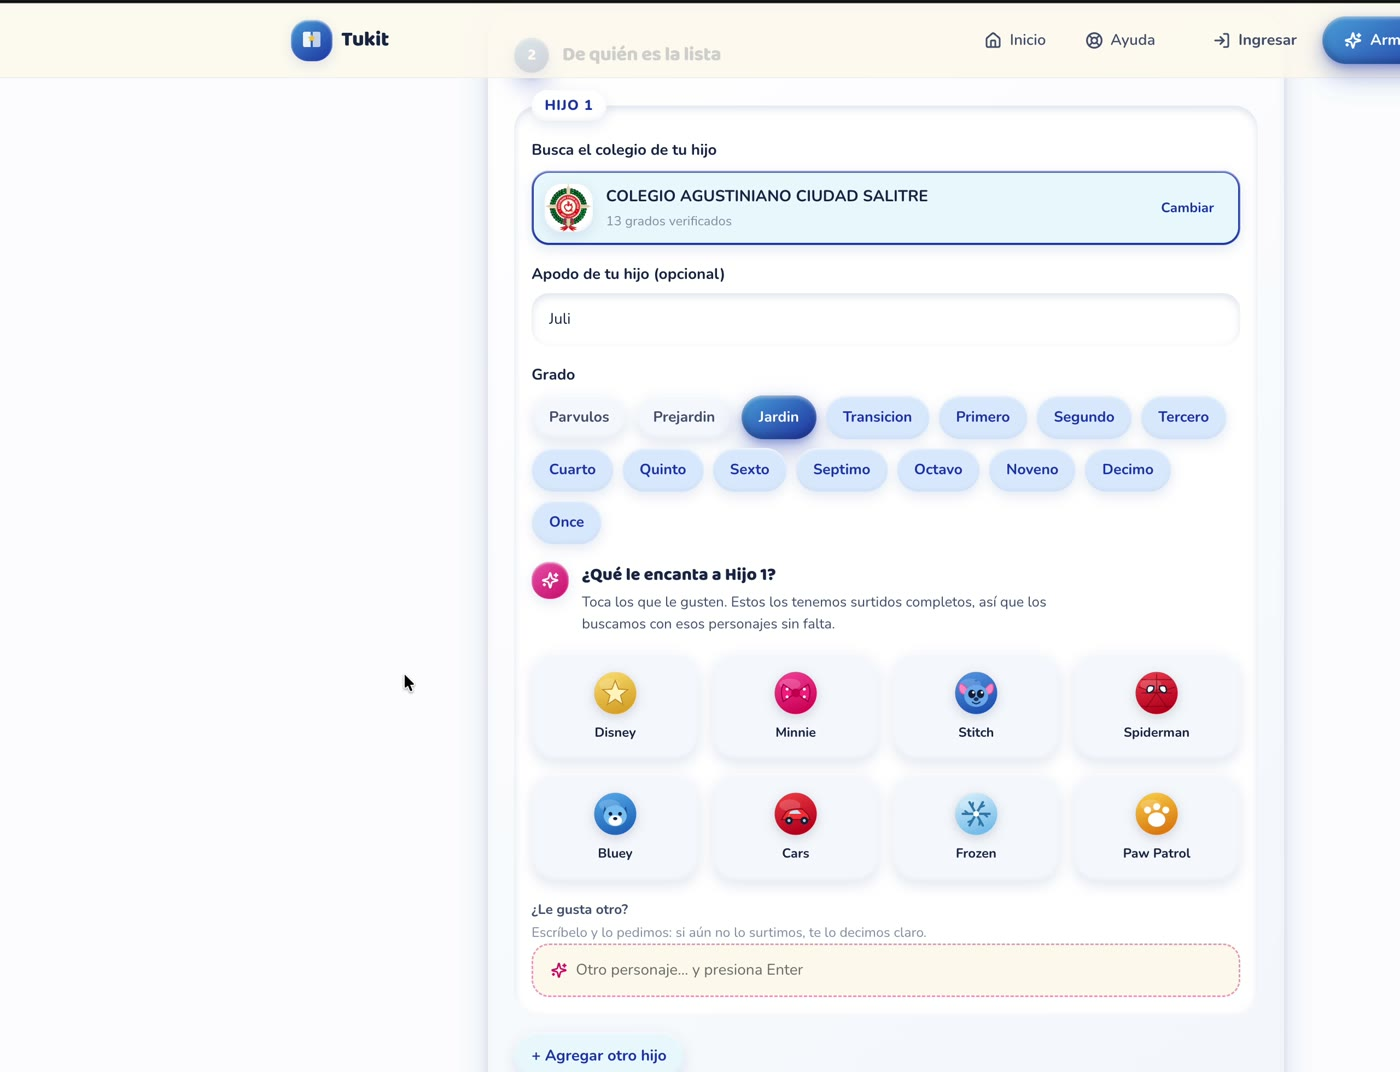
\includegraphics[width=0.32\textwidth]{img/producto/solicitud.jpg} &
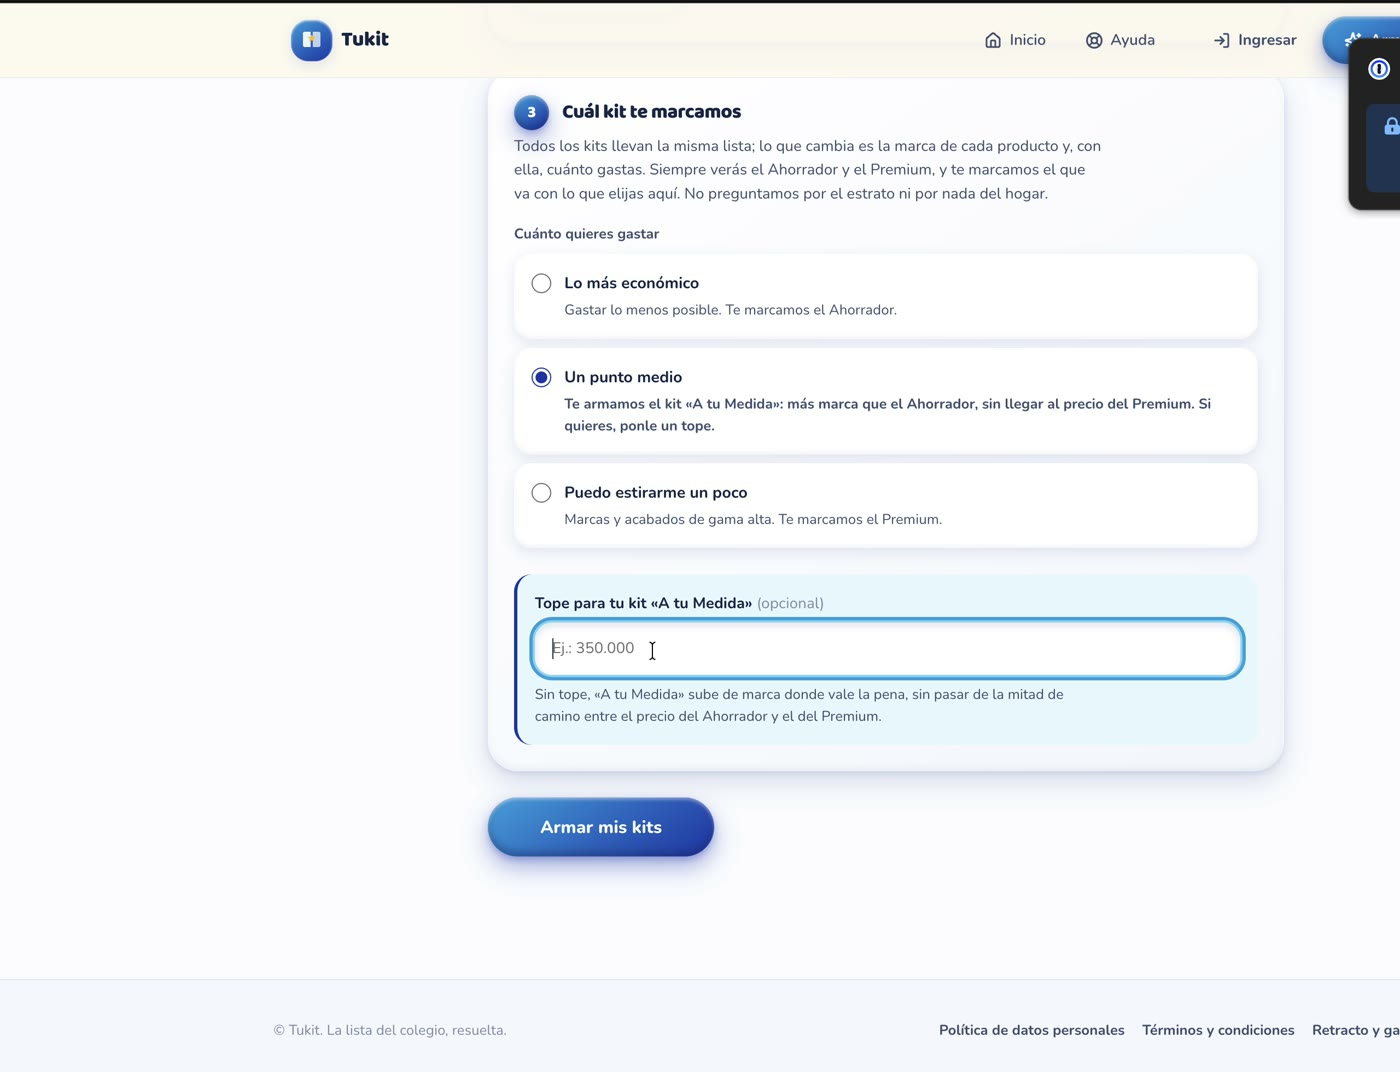
\includegraphics[width=0.32\textwidth]{img/producto/gasto.jpg} \\
\footnotesize (a) Portada & \footnotesize (b) De quién es la lista & \footnotesize (c) Opción de gasto \\[3pt]
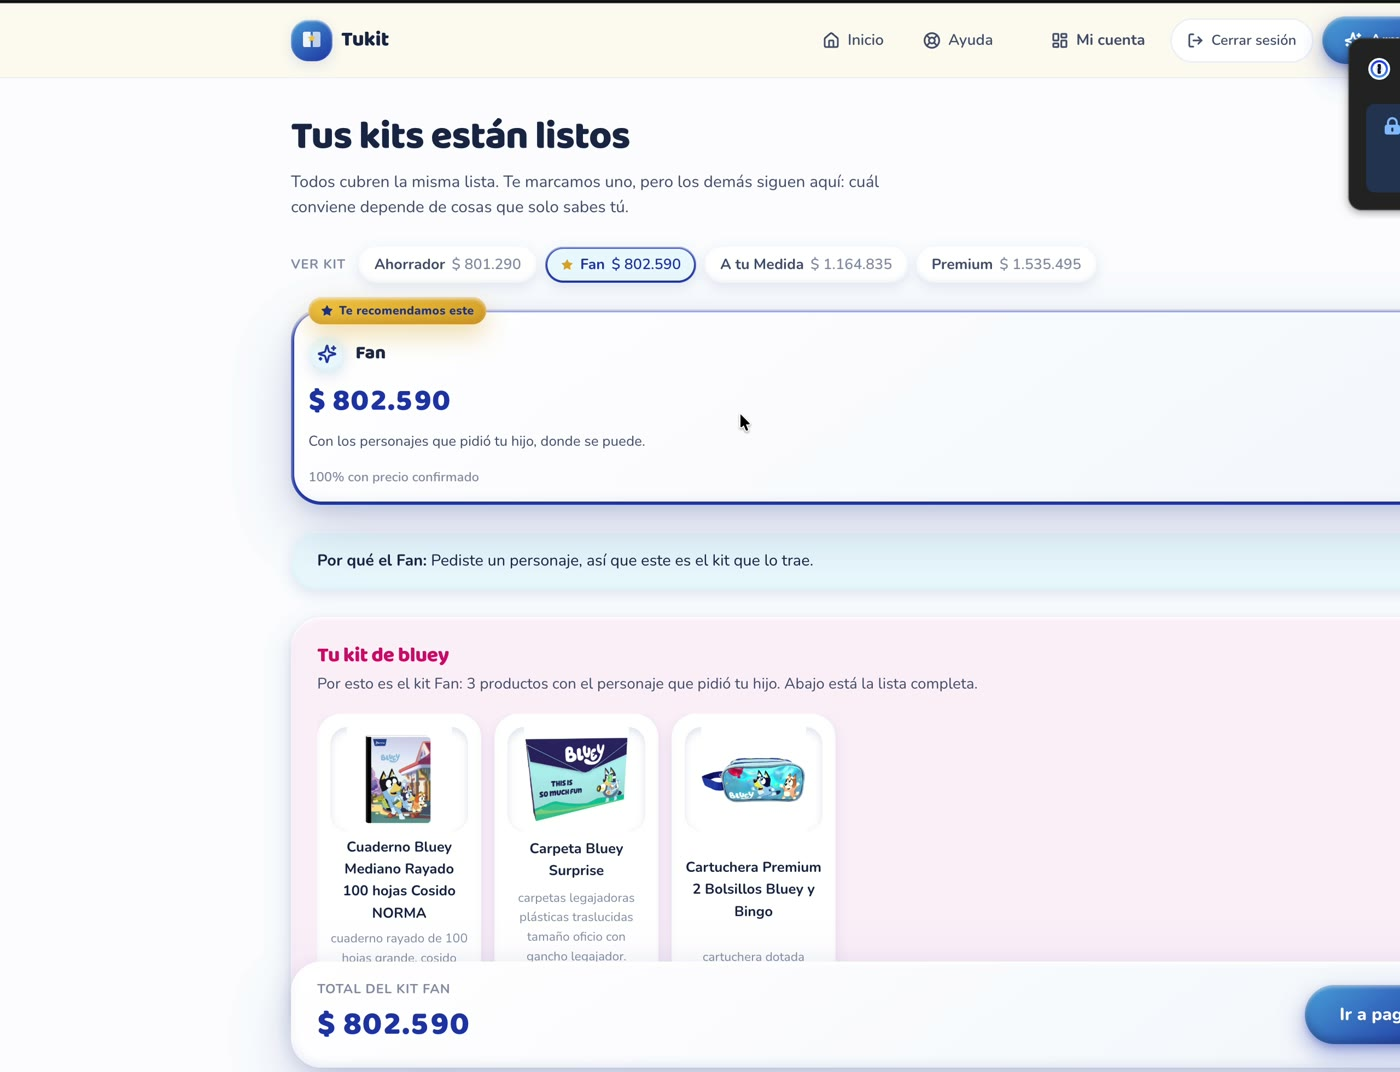
\includegraphics[width=0.32\textwidth]{img/producto/kits.jpg} &
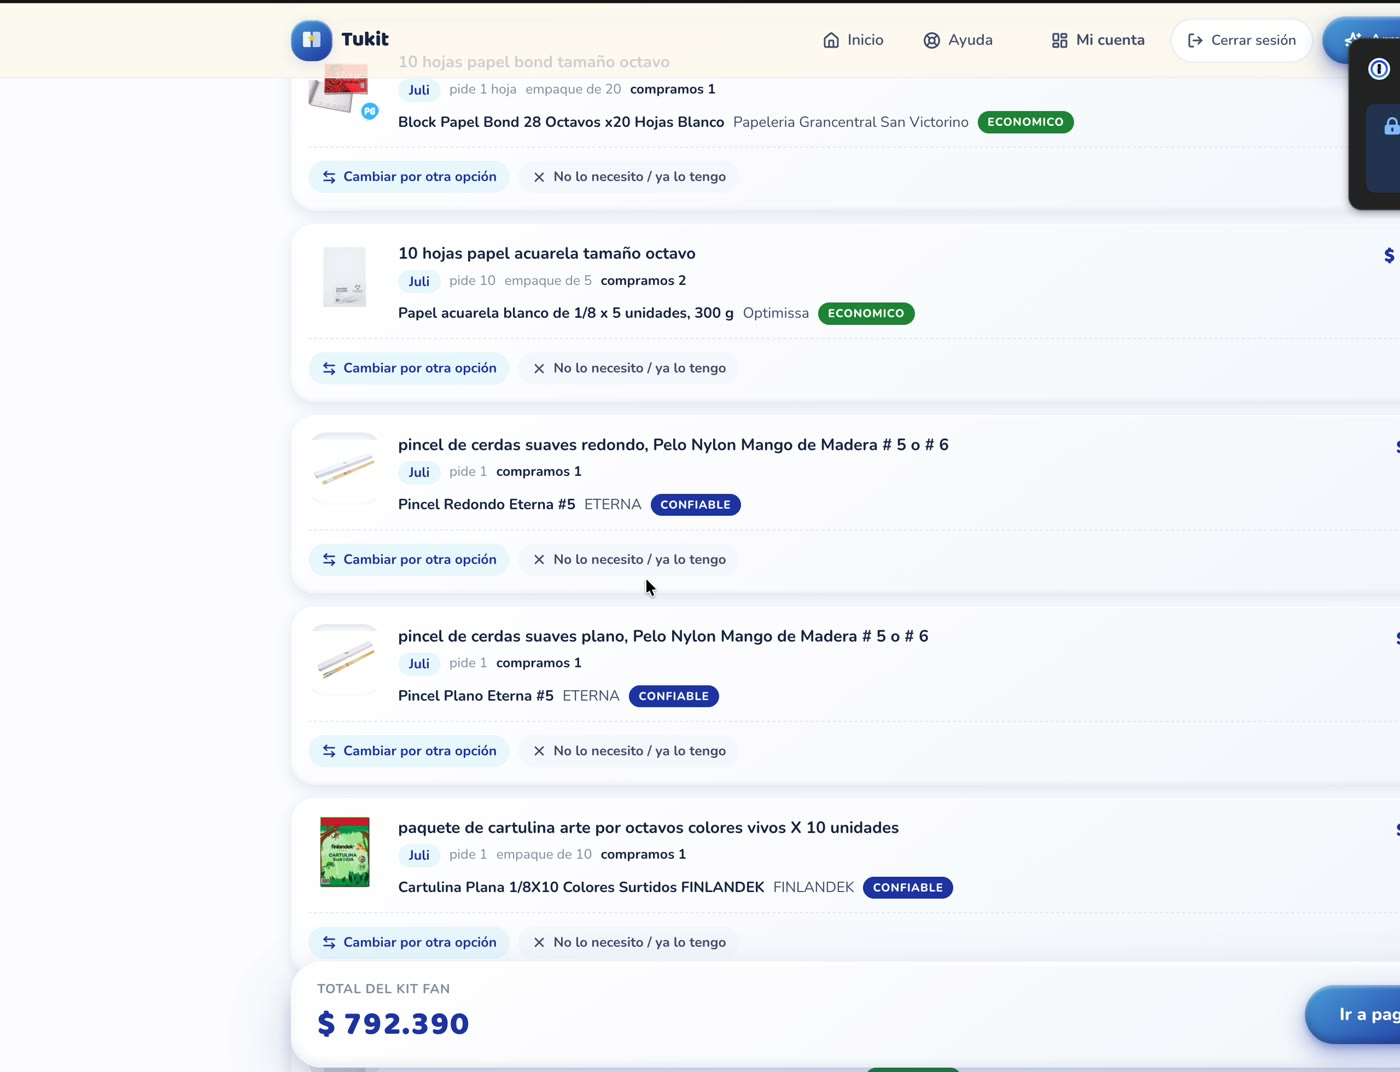
\includegraphics[width=0.32\textwidth]{img/producto/lineas.jpg} &
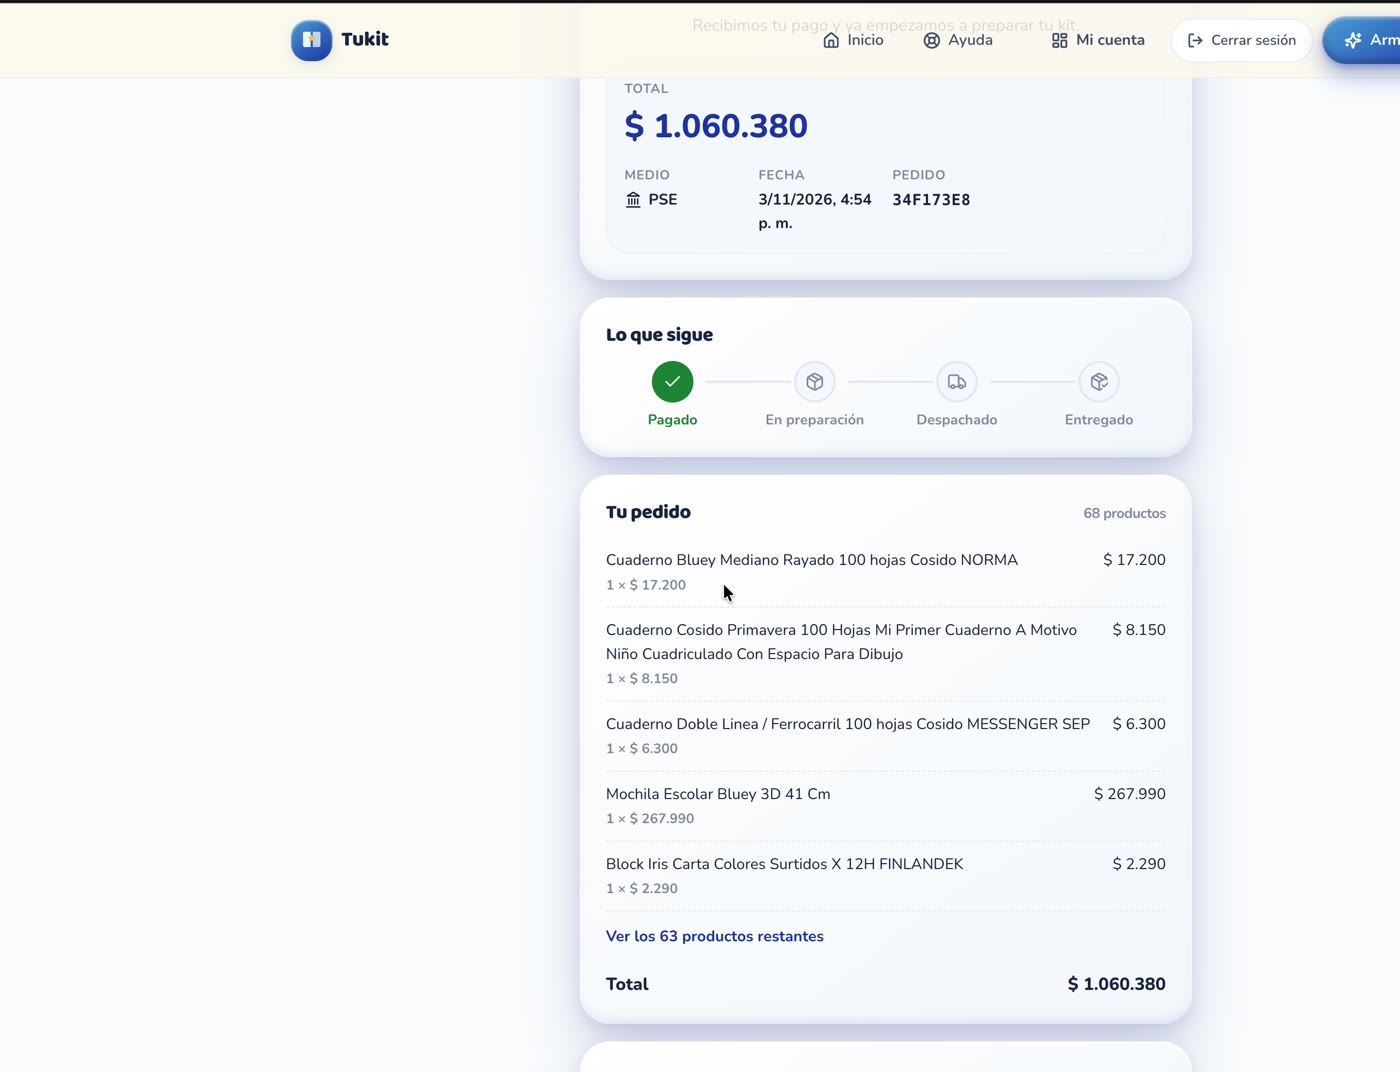
\includegraphics[width=0.32\textwidth]{img/producto/pago.jpg} \\
\footnotesize (d) Los kits & \footnotesize (e) Cambiar o quitar & \footnotesize (f) Pago aprobado \\
\end{tabular}
\caption[Recorrido del acudiente en la aplicación web.]{Recorrido del acudiente en la aplicación
web, capturado en la versión usada en el OE5 (versión \texttt{b6b6fe7}, pago simulado). La
Figura~\ref{fig:producto-equipo} (Anexo~\ref{anx:figuras}) muestra la cuenta del acudiente y la
revisión del kit por el equipo.}
\label{fig:recorrido}
\end{figure}

La Tabla~\ref{tab:requisito-pantalla} une cada pantalla con el requisito que atiende y con la prueba
que lo verifica, de modo que la figura no sea solo ilustrativa.

\begin{table}[htbp]
\centering
\scriptsize
\caption{Pantalla, requisito y prueba que la verifica.}
\label{tab:requisito-pantalla}
\begin{tabularx}{\textwidth}{@{}lXX@{}}
\toprule
Pantalla & Qué atiende & Cómo se verificó \\
\midrule
(b) De quién es la lista & Elegir colegio, grado y gustos por hijo; un pedido por hogar & Pruebas de identidad y T1 y T2 del OE5 \\
(c) Opción de gasto & Prioridad y tope como restricción dura (ADR 0029, 0030) & Pruebas del optimizador y T2 \\
(d) Los kits & De dos a cuatro kits del mismo frente (ADR 0030), con uno recomendado (MAUT) & Igualdad con el óptimo exacto y T4 \\
(e) Cambiar o quitar & Descarte y cambio por opciones del mismo concepto (ADR 0028) & Pruebas de comercio y T5 \\
(f) Pago aprobado & Pago en el widget, confirmación idempotente (ADR 0025, 0033) & Recorrido con pago simulado y T6 y T7 \\
Revisión del equipo & Cada lista nueva se revisa antes de publicarla (PE-04) & Pruebas de la cola y T3 \\
\bottomrule
\end{tabularx}
\end{table}

El panel de administración recibió, en la misma integración, el detalle completo del pedido (con el
estado del retracto y el despacho por transportadora), la bandeja de tickets con filtros,
conversación, respuesta, cambio de estado y vínculo al pedido, y un mapa de entregas pendientes en
logística con el consolidado por colegio. El mapa usa OpenStreetMap con Leaflet; las direcciones se
geocodifican en el servidor con Nominatim, a una consulta por segundo, una sola vez por dirección y
con caché también de las que no se encuentran, para cumplir su política de uso.

El flujo de pago se probó con la pasarela en modo simulado (\texttt{WOMPI\_MODO=falso}), que es
el modo por omisión del sistema. La prueba con las llaves del entorno de pruebas (\emph{sandbox})
de Wompi queda pendiente\pendienteEvidencia{pago de extremo a extremo en el sandbox de Wompi}, y
el cobro con dinero real depende del despliegue productivo (Sección~\ref{sec:trabajo-futuro}).

% Contenido que llega de otras sesiones (calibracion y MAUT; NL2C).
\subsection{Optimización y calibración}
\label{sec:optimizacion-cal}

La resolución asignó cada renglón a un concepto (Sección~\ref{sec:algoritmo-resolucion}), y cada concepto
reúne uno o más productos candidatos. Eso no basta para entregar un kit: falta escoger un producto por
renglón, y esa elección es un compromiso entre costo, marca, disponibilidad y personaje. Este problema es
la fase de modelado (\emph{Modeling}) de CRISP-DM en la Fase~4 (OE4).  La sección lo formaliza, lo
resuelve y lo calibra; sus límites se reúnen en la Sección~\ref{sec:amenazas}. La
Figura~\ref{fig:calibracion-flujo} resume el proceso de calibración, y cada caja remite a la gráfica o a la
tabla del Anexo~\ref{anx:calibracion}, que queda como consulta.

\begin{figure}[!htb]
\centering
\resizebox{\textwidth}{!}{% Proceso de calibración del optimizador, de los datos a la evaluación en las listas de prueba.
% Misma paleta que c4-contenedores.tex. Las cifras salen de los macros \cal* de sections/cifras_calibracion.tex.

\definecolor{tkPerF}{HTML}{FFF0B8}\definecolor{tkPerB}{HTML}{9A7B00}
\definecolor{tkAppF}{HTML}{CFE2F7}\definecolor{tkAppB}{HTML}{1F4E86}
\definecolor{tkProcF}{HTML}{D3EDD0}\definecolor{tkProcB}{HTML}{2E6B2B}
\definecolor{tkExtF}{HTML}{FAD7B5}\definecolor{tkExtB}{HTML}{A8500F}
\definecolor{tkInfF}{HTML}{DEDEDE}\definecolor{tkInfB}{HTML}{4D4D4D}
\definecolor{tkBdF}{HTML}{CDEBEB}\definecolor{tkBdB}{HTML}{1C6E6E}
\definecolor{tkMqF}{HTML}{E2D6F4}\definecolor{tkMqB}{HTML}{5B2E99}
\begin{tikzpicture}[x=1cm, y=1cm, font=\scriptsize,
  per/.style={draw, thick, rounded corners=7pt, align=center, draw=tkPerB, fill=tkPerF, inner sep=3pt, minimum height=7mm},
  cont/.style={draw, rounded corners=2pt, align=center, draw=tkAppB, fill=tkAppF, inner sep=2pt, minimum height=8mm},
  proc/.style={draw, rounded corners=2pt, align=center, draw=tkProcB, fill=tkProcF, inner sep=2pt, minimum height=7mm},
  ext/.style={draw, rounded corners=2pt, align=center, draw=tkExtB, fill=tkExtF, inner sep=2pt, minimum height=7mm},
  infra/.style={draw, rounded corners=2pt, align=center, draw=tkInfB, fill=tkInfF, inner sep=2pt, minimum height=7mm},
  bd/.style={draw, cylinder, shape border rotate=90, aspect=0.22, align=center, fill=tkBdF,
    minimum width=1.25cm, draw=tkBdB, minimum height=8mm, inner sep=1pt},
  grupo/.style={draw=black!55, rounded corners=3pt, fill=black!4},
  http/.style={-{Stealth[length=1.6mm]}, semithick},
  evt/.style={-{Stealth[length=1.6mm]}, densely dashed, semithick},
  cola/.style={-{Stealth[length=1.6mm]}, semithick, draw=tkMqB},
  hueco/.style={draw=white, line width=2.8pt},
  paso/.style={circle, draw, fill=white, inner sep=0.5pt, font=\scriptsize\bfseries, minimum size=4.4mm},
  rot/.style={font=\scriptsize, fill=white, inner sep=1pt},
  etapa/.style={draw, thick, rounded corners=3pt, align=left, inner sep=4pt, text width=4.7cm, minimum height=3.1cm, anchor=north west},
  tit/.style={font=\footnotesize\bfseries, anchor=north west, inner sep=0pt},
  ref/.style={font=\scriptsize\itshape, anchor=south west, inner sep=0pt}]
\def\caja#1#2#3#4#5#6{% color, posición, título, cuerpo, dónde se ve, nombre
  \node[etapa, draw=tk#1B, fill=tk#1F] (#6) at #2 {};
  \node[tit] at ([shift={(4pt,-4pt)}]#6.north west) {#3};
  \node[anchor=north west, text width=4.4cm, align=left, inner sep=0pt] at ([shift={(4pt,-0.75cm)}]#6.north west) {#4};
  \node[ref] at ([shift={(4pt,4pt)}]#6.south west) {#5};}
\caja{Bd}{(0,0)}{1. Datos y pliegues}{\calListas{} listas de \calColegios{} colegios.\\
  Prueba: \calColegiosPrueba{} colegios, \calHVListas{} listas, apartadas antes de mirar resultados.\\
  Ajuste: \calPliegues{} pliegues por colegio, \calCVListas{} listas.}{Tabla~\ref{tab:calopt-rejilla}}{p1}
\caja{App}{(5.7,0)}{2. Umbral: exacto o NSGA-II}{\calSubproblemas{} subproblemas medidos.\\
  Ajuste del exacto: $t\approx\calConstante\,S^{\calExponente}$ s.\\
  Cruce de los dos métodos y umbral $\Lambda=\calLimite$.}{Fig.~\ref{fig:calibracion-graficas}a, Tab.~\ref{tab:calopt-umbral}}{p2}
\caja{App}{(11.4,0)}{3. Rejilla $a$, $b$}{$a,b\in\{\calFactores\}$.\\
  Se elige la configuración más barata a menos de \calUmbralHV{} del mejor hipervolumen.\\
  Elegida: $a=b=\calA$.}{Fig.~\ref{fig:calibracion-graficas}b, Tab.~\ref{tab:calopt-rejilla}}{p3}
\caja{Mq}{(0,-4.3)}{4. Pesos MAUT desde la P21}{\calEncuestados{} acudientes ordenan cuatro criterios.\\
  Precio \calWPrecio, marca \calWMarca, calidad \calWCalidad, personaje \calWPersonaje.\\
  IC 95\,\% por \emph{bootstrap}.}{Fig.~\ref{fig:calibracion-graficas}c}{p4}
\caja{Mq}{(5.7,-4.3)}{5. Sensibilidad Dirichlet}{\calSensListas{} listas y \calSensPerturbaciones{} sorteos de pesos dentro de los intervalos.\\
  El kit recomendado se mantiene en al menos \calSensICMin{} de los sorteos.}{Fig.~\ref{fig:calibracion-graficas}d, Tab.~\ref{tab:calopt-sensibilidad}}{p5}
\caja{Proc}{(11.4,-4.3)}{6. Umbral de similitud $\tau$}{$\tau=0{,}75$ se evalúa y se conserva.\\
  \calTauPares{} pares de \calTauColegios{} colegios; AUC \calTauAUC, precisión \calTauPrecision.}{Fig.~\ref{fig:tau-clasificacion}, Sec.~\ref{sec:recuperacion}}{p6}
\caja{Ext}{(0,-8.6)}{7. Evaluación en prueba}{Hipervolumen relativo al frente exacto: \calHVFrente{} en las \calHVListas{} listas; \calPruebaElegidaHV{} en las \calHVListasNsga{} con NSGA-II.\\
  Un solo kit cubre menos: MAUT \calHVMAUTPesos, Ahorrador \calHVAhorrador, Premium \calHVPremium.}{Fig.~\ref{fig:calibracion-graficas}e, Tab.~\ref{tab:calopt-hv}}{p7}
% Flechas del proceso
\draw[http] (p1.east |- 0,-1.5) -- (p2.west |- 0,-1.5);
\draw[http] (p2.east |- 0,-1.5) -- (p3.west |- 0,-1.5);
\draw[http] (p3.south) -- ++(0,-0.55) -| node[rot, pos=0.25] {configuración elegida} (p4.north);
\draw[http] (p4.east |- 0,-5.8) -- (p5.west |- 0,-5.8);
\draw[http] (p5.east |- 0,-5.8) -- (p6.west |- 0,-5.8);
\draw[http] (p6.south) -- ++(0,-0.55) -| node[rot, pos=0.25] {pesos y $\tau$ fijados} (p7.north);
% Leyenda
\def\tkley#1#2#3#4{\node[#1, minimum width=7mm, minimum height=4.2mm, inner sep=0pt, text width=7mm] at #2 {};
  \node[anchor=west, font=\scriptsize, inner sep=1pt] at ([xshift=4.5mm]#2) {#3};}
\node[draw=black!40, rounded corners=2pt, anchor=north west, minimum width=10.2cm, minimum height=1.9cm,
  inner sep=0pt] (cajaley) at (6.2,-8.6) {};
\node[anchor=north west, font=\scriptsize\bfseries] at ([shift={(2mm,-1mm)}]cajaley.north west) {Leyenda};
\begin{scope}[shift={(cajaley.north west)}]
\node[draw=tkBdB, fill=tkBdF, rounded corners=2pt, minimum width=7mm, minimum height=4.2mm] at (0.9,-0.75) {};
\node[anchor=west, font=\scriptsize] at (1.4,-0.75) {Datos};
\node[draw=tkAppB, fill=tkAppF, rounded corners=2pt, minimum width=7mm, minimum height=4.2mm] at (3.2,-0.75) {};
\node[anchor=west, font=\scriptsize] at (3.7,-0.75) {Optimizador};
\node[draw=tkMqB, fill=tkMqF, rounded corners=2pt, minimum width=7mm, minimum height=4.2mm] at (6.2,-0.75) {};
\node[anchor=west, font=\scriptsize] at (6.7,-0.75) {Pesos MAUT};
\node[draw=tkProcB, fill=tkProcF, rounded corners=2pt, minimum width=7mm, minimum height=4.2mm] at (0.9,-1.4) {};
\node[anchor=west, font=\scriptsize] at (1.4,-1.4) {Umbral $\tau$};
\node[draw=tkExtB, fill=tkExtF, rounded corners=2pt, minimum width=7mm, minimum height=4.2mm] at (3.2,-1.4) {};
\node[anchor=west, font=\scriptsize] at (3.7,-1.4) {Evaluación};
\draw[http] (6.0,-1.4) -- +(0.7,0); \node[anchor=west, font=\scriptsize] at (6.8,-1.4) {Paso siguiente};
\end{scope}
\end{tikzpicture}
}
\caption[Proceso de calibración del optimizador.]{Proceso de calibración del optimizador, de los
datos a la evaluación en las listas de prueba. Cada caja trae su cifra principal y la figura o tabla
donde se ve.}
\label{fig:calibracion-flujo}
\end{figure}

\paragraph{Análisis del problema.} Cada producto que satisface un renglón comprable se llama \emph{candidato}. Sea $n$ el número de
\emph{líneas decidibles}, es decir, los renglones con al menos un candidato admisible, y sea $C_i$
el conjunto de candidatos de la línea $i$. Un kit es una asignación
$\mathbf{x}=(x_1,\dots,x_n)$ con $x_i\in C_i$, y el espacio de búsqueda tiene
$S=\prod_{i=1}^{n}|C_i|$ asignaciones, de modo que crece de forma exponencial con las líneas:
basta con dos candidatos por línea para que $S\geq 2^n$. Cada kit se evalúa con cuatro objetivos
($M=4$): el costo $f_1$, que se minimiza, y la fidelidad de marca $f_2$, la disponibilidad $f_3$ y
el personaje $f_4$, normalizados en $[0,1]$, que se maximizan. Como el candidato más barato rara
vez es el de mejor marca, no existe en general un kit que sea el mejor en los cuatro. Por eso se
busca el \emph{frente de Pareto} $\mathcal{P}$, el conjunto de kits que ningún otro domina, donde
un kit domina a otro si no es peor en ningún objetivo y es mejor en al menos uno. Como el acudiente compra un solo kit, sobre $\mathcal{P}$ hay que escoger un
punto según sus preferencias. Las \calListas{} instancias del banco salen de 174 listas de
\calColegios{} colegios: \calListasNsga{} superan el umbral de enumeración, \calListasExacto{} quedan
por debajo, y el espacio más grande es del orden de $10^{\calEspacioMaxLog}$.

\paragraph{Modelo formal.} Para fijar el problema se usan variables de decisión binarias. Sea
$x_{i,p}\in\{0,1\}$ igual a 1 si se elige el producto $p$ para la línea decidible $i$, con
$\sum_{p\in C_i}x_{i,p}=1$ para cada $i$, de modo que cada línea recibe exactamente un producto. El código usa una forma equivalente: la variable de la línea $i$ es el índice entero del candidato,
en $\{0,\dots,|C_i|-1\}$, que es la que recibe NSGA-II. Las restricciones duras son
tres y actúan en momentos distintos.
\begin{enumerate}[label=\textbf{R\arabic*.},leftmargin=*,itemsep=1pt,topsep=2pt]
\item \emph{Filtros del acudiente, antes del frente} (\texttt{aplicar\_filtros\_duros}). Si
el acudiente excluye una marca, se retira de $C_i$ todo candidato de esa marca, salvo que el colegio la
exija en el renglón; si pide solo productos disponibles, se retiran los
candidatos sin oferta vigente. Si $C_i$ queda vacío, la línea pasa a ser un hueco del catálogo con un
mensaje. Se hace antes porque una restricción dura no debe
competir como un peso más.
\item \emph{Admisibilidad} (\texttt{\_admisibles}). Una línea es decidible si no es informativa y
tiene candidatos. Entre ellos se prefieren los que cumplen el atributo exigido por el colegio; si
ninguno lo cumple, entran todos.
\item \emph{Tope de gasto y sobreprecio, después del frente} (\texttt{\_tope},
\texttt{elegir\_recomendado\_maut}). El tope $B$ es el presupuesto declarado, sin estirarlo con el
sobreprecio, y se exige $f_1(\mathbf{x})\leq B$ y $f_1(\mathbf{x})\leq(1+\sigma)\,c_{\min}$, con $\sigma$ el
sobreprecio aceptado y $c_{\min}$ el menor costo entre los kits del frente con la máxima disponibilidad $f_3$,
filtro que se aplica antes para recomendar solo lo que está disponible hoy. Se aplican
sobre el frente completo, porque recortarlo antes escondería opciones que el acudiente aún puede querer ver.
\end{enumerate}
La cantidad por empaque entra en el costo. Si la línea pide $q_i$ unidades y el producto $p$ trae $e_p$
unidades por empaque, se compran $u_{i,p}=\lceil q_i/e_p\rceil$ empaques (\texttt{unidades\_a\_comprar}),
que es cero si $q_i\leq 0$. Con $\pi_p$ el precio del empaque, $\rho_p\in\{0,1,2\}$ el nivel de marca
(económico, confiable, premium), $\kappa_p=1$ si el producto trae el personaje buscado y $d_p=1$ si
tiene precio, los cuatro objetivos de $\mathbf{x}$ son
\begin{align}
f_1(\mathbf{x})&=\sum_{i}\sum_{p\in C_i:\,d_p=1}x_{i,p}\,\pi_p\,u_{i,p}, &
f_2(\mathbf{x})&=\frac{1}{2n}\sum_{i}\sum_{p}x_{i,p}\,\rho_p,\label{eq:f1f2}\\
f_3(\mathbf{x})&=\frac{1}{n}\sum_{i}\sum_{p}x_{i,p}\,d_p, &
f_4(\mathbf{x})&=\frac{1}{n}\sum_{i}\sum_{p}x_{i,p}\,\kappa_p.\label{eq:f3f4}
\end{align}
El costo $f_1$ está en pesos y suma solo los productos con precio, de modo que la
falta de precio baja $f_3$ y no abarata el kit. Los otros tres son promedios por línea en $[0,1]$:
$f_2$ divide el nivel de marca entre su máximo, 2; $f_3$ es la fracción de líneas
disponibles hoy; y $f_4$ es la fracción de líneas con el personaje pedido, o con cualquiera
si no se pidió ninguno. El problema es entonces minimizar
$(f_1,-f_2,-f_3,-f_4)$ sobre las asignaciones que cumplen R1 y R2; R3 se aplica al escoger el punto.

\paragraph{Diseño: entradas y salidas.} La Tabla~\ref{tab:es-optimizador} define los tipos.

\begin{table}[H]
\centering\footnotesize
\caption{Entradas y salidas del optimizador del kit.}
\label{tab:es-optimizador}
\begin{tabularx}{\textwidth}{@{}p{2.6cm}p{4.4cm}X@{}}
\toprule
Elemento & Tipo & Descripción \\
\midrule
Entrada $C_1,\dots,C_n$ & conjuntos no vacíos de candidatos & Cada candidato trae precio en pesos (o ninguno), unidades por empaque, nivel de marca en $\{0,1,2\}$ y personaje; cada línea trae su cantidad \\
Entrada $\mathbf{w}$ & cuatro reales no negativos & Pesos de precio, marca exigida, calidad y personaje; por omisión, los de la encuesta \\
Entradas $B$ y $\sigma$ & entero positivo y real en $[0,1]$, opcionales & Tope de gasto por hijo y sobreprecio aceptado sobre el kit más barato \\
Parámetros & entero $\Lambda$ y semilla $s$ & Umbral de enumeración y semilla del generador, para que el frente sea reproducible \\
Salida $\mathcal{P}$ & kits no dominados con su vector $(f_1,\dots,f_4)$ & Exacto si $S\leq\Lambda$ y aproximado si $S>\Lambda$, ordenado por costo \\
Salida $\mathbf{x}^\star$ & kit de $\mathcal{P}$ o nulo & Kit recomendado; nulo si ninguno cumple el tope y el sobreprecio \\
\bottomrule
\end{tabularx}
\end{table}

\paragraph{Estrategia algorítmica.} La estrategia tiene dos fases: primero se calcula el frente y
después se escoge un punto sobre él. Para la primera fase, el tamaño del espacio decide el método.
Si $S\leq\Lambda$, se enumeran las $S$ asignaciones y se conservan las no dominadas, lo que da el
frente exacto sin depender de ninguna semilla. Si $S>\Lambda$, se corre NSGA-II
\citep{deb_fast_2002} sobre pymoo \citep{blank_pymoo_2020}, un algoritmo evolutivo que mantiene una
\emph{población} de $N$ kits y, en cada una de las $G$ \emph{generaciones}, produce descendientes
por cruce y mutación y conserva los mejores. La población inicial se siembra con los kits que arma una regla sencilla para cada perfil, de modo que
el frente aproximado nunca queda por debajo de ellos. El algoritmo conserva los mejores kits según su
rango de dominancia y, entre los de igual rango, los más alejados de sus vecinos (la distancia de
apiñamiento), para que el frente no se concentre en una sola zona. La corrida termina tras un número
fijo de generaciones para que la misma semilla reproduzca el mismo frente.

La segunda fase usa la teoría de la utilidad multiatributo (MAUT) \citep{keeney_decisions_1976}
\emph{a posteriori}, es decir, primero se calcula el frente y después las preferencias escogen sobre
él \citep{miettinen_nonlinear_1999}. Para cada objetivo se define una utilidad $u_j$, lineal entre
el peor y el mejor valor que alcanza el frente, y la utilidad del kit es
$U=\hat w_{\mathrm{precio}}\,u_1+(\hat w_{\mathrm{marca}}+\hat w_{\mathrm{calidad}})\,u_2+\hat w_{\mathrm{personaje}}\,u_4$,
donde $\hat{\mathbf{w}}$ son los pesos renormalizados para que sumen 1. No entra $u_3$, porque la
disponibilidad ya se fijó en su máximo. La marca exigida y la
calidad pesan sobre la misma utilidad porque el frente mide ambas con el nivel de marca. La forma
aditiva supone \emph{independencia preferencial}, es decir, que la preferencia entre dos valores de
un criterio no depende de los valores de los demás, y ese supuesto se declara. En el código, esta
fase es la función \texttt{elegir\_recomendado\_maut}, y la regla de recomendación la usa para
decidir el Premium: lo marca cuando el acudiente acepta al menos un 10\,\% de sobreprecio y MAUT lo
prefiere al Ahorrador. El Algoritmo~\ref{alg:frente-maut} reúne las dos fases.

Fuera del frente, el kit Fan se arma con una regla de presentación que se aplica después de
calcularlo. Para cada hijo y concepto, el producto de personaje va una vez en la línea donde mejor
encaja sin contradecir sus atributos exigidos, y solo se repite donde la línea pide surtido. Su costo
es $O(n\cdot a)$, con $a$ el número de atributos exigidos por línea.

\begin{algorithm}[H]
\caption{Construcción del frente y selección del kit recomendado}
\label{alg:frente-maut}
\KwEntrada{candidatos $C_1,\dots,C_n$; pesos $\mathbf{w}$; tope $B$; sobreprecio $\sigma$; umbral $\Lambda$; semilla $s$}
\KwSalida{frente $\mathcal{P}$ y kit recomendado $\mathbf{x}^\star$ (o nulo)}
$S \leftarrow \prod_{i=1}^{n}|C_i|$\;
\uIf{$S\leq 1$}{\Return{(vacío, nulo)} \tcp*{no hay decisión que tomar}}
\uElseIf{$S\leq\Lambda$}{$\mathcal{P}\leftarrow$ no dominados de $\{\mathbf{F}(\mathbf{x}) : \mathbf{x}\in C_1\times\cdots\times C_n\}$ \tcp*{exhaustivo}}
\Else{
  $N\leftarrow\mathrm{par}(\min(100,\max(20,6n)))$;\quad $G\leftarrow\min(60,\max(15,10\log_{10}S))$\;
  $Q_0\leftarrow$ kits heurísticos por perfil, completados al azar con la semilla $s$ hasta $N$\;
  \For{$g = 1,\dots,G$}{
    $R\leftarrow Q_{g-1}\cup{}$ CruceYMutación$(Q_{g-1})$\;
    $Q_g\leftarrow$ los $N$ mejores de $R$ por frente no dominado y apiñamiento\;
  }
  $\mathcal{P}\leftarrow$ no dominados de $Q_G\cup Q_0$\;
}
$D\leftarrow$ kits de $\mathcal{P}$ con la máxima disponibilidad $f_3$ \tcp*{solo lo disponible}
$c_{\min}\leftarrow$ menor costo $f_1$ en $D$\;
$K\leftarrow\{\mathbf{x}\in D : f_1(\mathbf{x})\leq B,\ f_1(\mathbf{x})\leq(1+\sigma)\,c_{\min}\}$\;
\lIf{$K$ es vacío}{\Return{$(\mathcal{P}$, nulo$)$}}
\Return{$(\mathcal{P},\ \arg\max_{\mathbf{x}\in K}U(\mathbf{x}))$} \tcp*{empates: menor costo}
\end{algorithm}

\paragraph{Complejidad y comparación con el método exhaustivo.} El exhaustivo visita las $S$
asignaciones y evalúa en cada una $M$ objetivos, con un costo de $\Theta(S\cdot M)$ evaluaciones, y
luego filtra los $V\leq S$ vectores distintos comparándolos por pares, con un costo de $O(V^2M)$ en
el peor caso; su tiempo crece, por tanto, con el tamaño del espacio. NSGA-II, en cambio, ordena en
cada generación $2N$ individuos con un costo de $O(MN^2)$ \citep{deb_fast_2002}, así que su
total es $O(G\cdot M\cdot N^2)$, que no crece con $S$ más que por $G$; a cambio, el frente que devuelve es una
aproximación. MAUT recorre el frente un número constante de veces, con un costo de
$O(|\mathcal{P}|\,M)$, despreciable frente a la construcción del frente.

En esta comparación se omite el factor $n$ de
evaluar un kit, común a los dos métodos, y $G$ y $N$ crecen con $\log S$ y $n$. Para saber desde qué tamaño conviene NSGA-II se igualan los dos costos, con la población y las
generaciones típicas cerca del umbral ($n=\calNTipico$, $N=\calPobTipica$ y $G=\calGenTipica$). Si
domina el filtro en su peor caso, con $V=S$, la igualdad $S^2M=GMN^2$ da $S=N\sqrt{G}=252\approx
2^{\calSTeoricoLog}$. Si domina la evaluación, $SM=GMN^2$ da $S=GN^2=63.504\approx 2^{\calSCuadradoLog}$.
El cruce queda entre esos dos valores, y como las constantes de cada operación difieren, el umbral
se fijó con la medición.

Para medirlo se armaron \calSubproblemas{} subproblemas con líneas reales y espacios entre $2^{\calNivelMin}$
y $2^{\calNivelMax}$, y en cada uno se midió el tiempo de pared de los dos métodos. Un
ajuste por mínimos cuadrados en escala logarítmica sobre los \calSubproblemasExacto{} enumerados da $t_{\mathrm{exh}}(S)\approx\calConstante\cdot S^{\calExponente}$~s; el exponente es
mayor que 1 porque el filtro de no dominados crece más rápido que la evaluación. NSGA-II, con la
configuración elegida, tardó una mediana de \calTNsgaElegidaMediana~s, y el ajuste la alcanza en
$S\approx\calCruceElegida$, o en $S\approx\calCruceElegidaP$ si se toma el percentil 95 del ajuste.
Por eso se fijó $\Lambda=\calLimite=2^{\calLimiteLog}$, con los factores $a$ y $b$ de población y generaciones ya elegidos sobre las mismas
instancias (párrafo \emph{Calibración de las constantes}), entre los dos cruces y dentro del rango que
predice la teoría. Por debajo del umbral, la enumeración fue más rápida en
\calExactoGanaBajoElegida{} subproblemas y, por encima, solo en \calExactoGanaSobreElegida. La
diferencia de calidad es pequeña: sobre \calCorridasHV{} corridas, la razón de
\emph{hipervolumen}, el volumen del espacio de objetivos que domina un frente hasta un punto de
referencia \citep{zitzler_multiobjective_1999}, entre el frente de NSGA-II y el exacto tuvo mediana
\calRazonHVMediana{} y mínimo \calRazonHVMin, con los cuatro ejes normalizados en $[0,1]$ y la
referencia en 1,1.  El exhaustivo pasa de dos minutos cerca de $2^{\calNivelMaxExacto}$.

\paragraph{Calibración de las constantes.} Los experimentos corrieron con semillas fijas en un \calCPU{} de
\calNucleos{} núcleos con \calRAM~GiB de memoria, Python \calPython{} y pymoo \calPymoo. Los pesos por omisión salen de la pregunta P21 de la encuesta, que pide ordenar los cuatro
criterios: el primero recibe 4 puntos y el último 1, y el peso es el puntaje medio dividido entre 10.
Con \calEncuestados{} respuestas, y con intervalos del 95\,\% por \emph{bootstrap}
\citep{efron_bootstrap_1979} (un remuestreo de las mismas respuestas que mide cuánto cambiaría el peso
con otra muestra), los pesos son precio \calWPrecio{} [\calWPrecioBajo; \calWPrecioAlto],
marca exigida \calWMarca{} [\calWMarcaBajo; \calWMarcaAlto], calidad \calWCalidad{}
[\calWCalidadBajo; \calWCalidadAlto] y personaje \calWPersonaje{} [\calWPersonajeBajo;
\calWPersonajeAlto]. Como los tres primeros intervalos se solapan, la encuesta no permite ordenar precio, marca y
calidad entre sí, y solo el personaje queda claramente por debajo (Figura~\ref{fig:calibracion-graficas}c).

Las fórmulas de partida de la población y de las generaciones eran
\[N=\min(200,\max(40,12n)),\qquad G=\min(120,\max(30,20\log_{10}S)).\] La calibración multiplicó la primera por $a$ y la segunda por
$b$, con $a,b\in\{\calFactores\}$, y escogió la configuración más barata cuyo hipervolumen medio no
bajara más de \calUmbralHV{} del mejor de la rejilla. Los datos se partieron por colegio, porque dos grados
de un mismo colegio comparten productos y marcas, y mezclarlos entre ajuste y prueba inflaría el
resultado. Antes de mirar ningún resultado se apartaron \calColegiosPrueba{} colegios como prueba, con
\calHVListas{} listas, \calPrueba{} de ellas por encima del umbral de enumeración, que son las únicas que
miden a NSGA-II. Con el resto se hizo validación cruzada en \calPliegues{} pliegues, es decir,
\calPliegues{} grupos de colegios que se dejan fuera por turnos. El hipervolumen relativo es el del
frente de cada configuración dividido entre el del mejor frente de la rejilla de $(a,b)$. La regla eligió $a=b=\calA$,
que da en producción las fórmulas del Algoritmo~\ref{alg:frente-maut}, y al dejar fuera cada pliegue
eligió lo mismo en \calPlieguesIguales. En el conjunto de prueba, usado una sola vez, la elegida
obtuvo un hipervolumen relativo medio de \calPruebaElegidaHV{} contra \calPruebaActualHV{} de la de
partida, una diferencia de \calDifHV{} con intervalo [\calDifHVBajo; \calDifHVAlto]
y $p<0{,}001$ en la prueba de rangos con signo de Wilcoxon \citep{wilcoxon_individual_1945}. En la
peor lista la elegida llegó a \calPruebaElegidaHVMin{} contra \calPruebaActualHVMin{}. La
pérdida es pequeña, y el tiempo medio por lista bajó de \calPruebaActualT~s a \calPruebaElegidaT~s.

El umbral de similitud $\tau=0{,}75$ de la resolución se evaluó y se mantuvo en su valor por omisión,
porque la única fuente humana es un solo revisor y la validación cruzada agrupada, que sugiere un
$\tau$ entre \calTauCVMin{} y \calTauCVMax{}, tiene una muestra demasiado concentrada para moverlo
(Sección~\ref{sec:recuperacion}). Para ver cuánto depende la recomendación de los pesos, se sortearon dentro de sus intervalos de la
P21. El kit recomendado se mantuvo en el 96,5\,\%, el 98,6\,\% y el 94,6\,\% de los sorteos con
sobreprecios de 5, 10 y 20\,\%, y en la peor lista, con 20\,\%, bajó al 54\,\%.

Por último, en las \calHVListas{} listas de los colegios de prueba el frente de producción alcanzó
\calHVFrente{} del hipervolumen exacto, y \calPruebaElegidaHV{} en las \calHVListasNsga{} con NSGA-II
(en las otras ocho el frente es exacto). La Figura~\ref{fig:calibracion-graficas} muestra qué se vio y qué se
decidió. En (a) el tiempo de la enumeración exacta sube en línea recta en escala logarítmica y el de
NSGA-II se mantiene cerca de un segundo; las curvas se cruzan cerca de la línea punteada, y de ahí
salió $\Lambda$, mientras la razón de hipervolumen queda en 1 casi siempre. En (b), la estrella cumple
el piso de \calUmbralHV{} con la cuarta parte de las evaluaciones del rombo de partida, y por eso se
eligió. En (c), el personaje queda aparte y los otros tres pesos se solapan. En (d), la fracción de
sorteos con el mismo kit cae con la perturbación y con el sobreprecio, pero se mantiene sobre 0,7, así
que la recomendación es estable. En (e), un solo kit cubre una fracción menor del hipervolumen exacto
(\calHVMAUTPesos{} el elegido por MAUT, \calHVAhorrador{} el Ahorrador y \calHVPremium{} el Premium),
y por eso se entrega el frente completo.

\begin{figure}[p]
\centering
{\footnotesize\textbf{(a)}}\\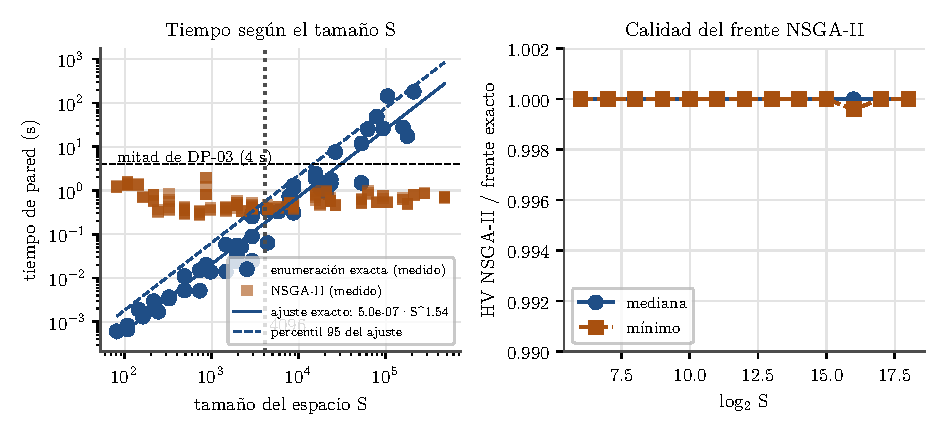
\includegraphics[width=0.82\linewidth]{img/calibracion/umbral.pdf}\\[1mm]
\begin{minipage}[t]{0.44\linewidth}\centering
{\footnotesize\textbf{(b)}}\\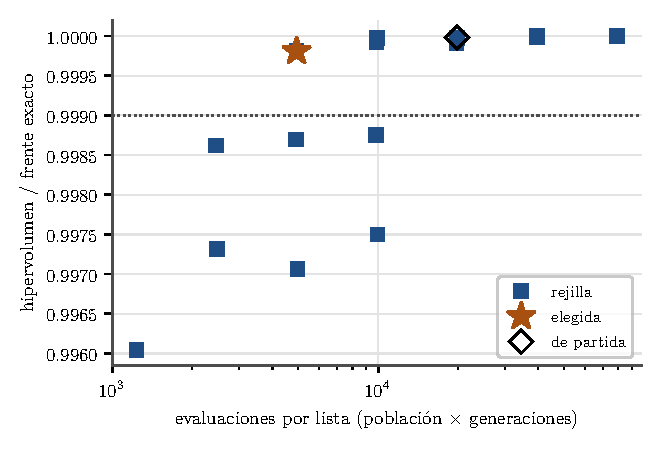
\includegraphics[width=\linewidth]{img/calibracion/rejilla.pdf}\end{minipage}\hfill
\begin{minipage}[t]{0.44\linewidth}\centering
{\footnotesize\textbf{(c)}}\\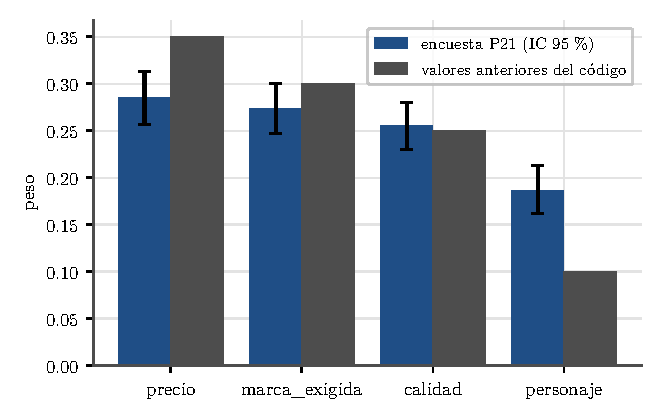
\includegraphics[width=\linewidth]{img/calibracion/pesos_p21.pdf}\end{minipage}\\[1mm]
\begin{minipage}[t]{0.44\linewidth}\centering
{\footnotesize\textbf{(d)}}\\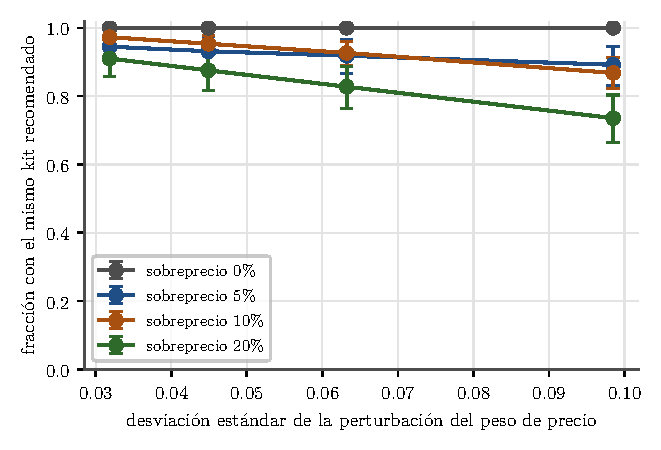
\includegraphics[width=\linewidth]{img/calibracion/sensibilidad.pdf}\end{minipage}\hfill
\begin{minipage}[t]{0.44\linewidth}\centering
{\footnotesize\textbf{(e)}}\\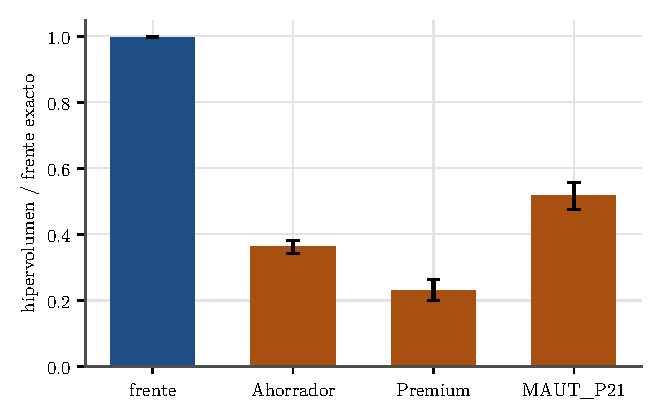
\includegraphics[width=\linewidth]{img/calibracion/hipervolumen_prueba.pdf}\end{minipage}
\caption[Gráficas de la calibración del optimizador.]{Calibración del optimizador. (a) Tiempo de la
enumeración exacta y de NSGA-II según el tamaño del espacio, y calidad del frente. (b) Rejilla de
población y generaciones. (c) Pesos de la P21 con su intervalo del 95\,\%. (d) Estabilidad del kit
recomendado bajo la perturbación de los pesos. (e) Hipervolumen relativo al frente exacto en las
listas de prueba.}
\label{fig:calibracion-graficas}
\end{figure}

Estos resultados tienen límites: los pesos salen de preferencias declaradas, la prueba tiene solo \calColegiosPrueba{} colegios, la calibración es retrospectiva y los tiempos son de una sola máquina; la Sección~\ref{sec:amenazas} los reúne con los del resto de la evidencia.

\subsection{Asistente en lenguaje natural (NL2C)}
\label{sec:nl2c}

El asistente convierte la frase de un acudiente en las restricciones del optimizador. Corresponde a las etapas de modelado y evaluación de CRISP-DM en las fases F3 y F4 y sigue la estructura de las secciones anteriores: problema, entradas y salidas, estrategia, seudocódigo, costo, resultados y límites. Las tablas
completas de la evaluación están en el Anexo~\ref{anx:nl2c}.

\paragraph{Análisis del problema.} La propuesta aprobada prometió que el acudiente pudiera
describir en español lo que quiere, por ejemplo «Minnie para mi hija, máximo 500 mil», en lugar de
llenar un formulario de opciones cerradas. A esa tarea se le llama NL2C (del inglés \emph{natural
language to constraints}): transformar un texto en el objeto de restricciones que un programa ya
consume, que aquí es el optimizador de la Sección~\ref{sec:optimizacion-cal}. El texto $t$ es una
cadena corta, ambigua y con errores de ortografía, y la salida es la terna
$\mathcal{R}=\langle F,W,P\rangle$ de filtros duros, pesos y preferencias, con los dominios de la
Tabla~\ref{tab:nl2c-dominios}. Un campo que el acudiente no menciona queda en su valor por omisión,
y uno que menciona fuera de dominio se lleva al dominio y se le avisa. Dos condiciones fijan el
diseño. La primera es que $t$ y el texto de la lista los puede escribir un atacante, de modo que
ninguno de los dos puede cambiar qué acciones ejecuta el sistema \citep{greshake2023indirect}. La
segunda es que un error le cuesta dinero al acudiente, por lo que nada se aplica sin su
confirmación. Las reglas fijas no bastan, porque los nombres de personajes y marcas son un
vocabulario abierto y una frase como «calidad primero y precio después» fija los pesos pero no el
estilo de gasto.

\begin{table}[H]
\centering\footnotesize
\caption{Dominio de los campos de $\mathcal{R}$. Fuente: constantes de \texttt{nl2c.py}.}
\label{tab:nl2c-dominios}
\begin{tabularx}{\textwidth}{@{}p{1.2cm}p{4.2cm}X@{}}
\toprule
Grupo & Campo & Dominio \\
\midrule
$F$ & \texttt{presupuesto\_max\_cop} & vacío o entero en $[50.000;\ 3.000.000]$ pesos por hijo \\
 & \texttt{marcas\_excluidas}, \texttt{solo\_disponibles} & hasta 10 cadenas de 1 a 40 caracteres; verdadero o falso \\
$W$ & cuatro pesos & cada $w_i\in[0{,}05;\ 0{,}60]$ y $\sum w_i=1$ \\
$P$ & \texttt{personajes}, \texttt{estilo\_gasto} & hasta 3 del catálogo; económico, punto medio o estirarse \\
\bottomrule
\end{tabularx}
\end{table}

\paragraph{Diseño: entradas y salidas.} Las entradas son el texto $t$, de a lo más 1.000 caracteres
después de sanearlo, el catálogo de personajes $\mathcal{C}_P$, con hasta 60 nombres, y una lista
blanca de ocho componentes de interfaz. Para pedir cambios sobre un kit se agrega el kit, con hasta
80 renglones. Las salidas son $\mathcal{R}$ validada, la lista de ajustes que hizo el servidor, la
especificación de la interfaz que se le muestra al acudiente y un estado, que puede ser propuesta,
sin acción, inválido o sin servicio. Si el estado es propuesta, $\mathcal{R}$ cumple la
Tabla~\ref{tab:nl2c-dominios}, todo texto libre de $\mathcal{R}$ aparece en $t$ y nada se aplica
antes de que el acudiente confirme.

\paragraph{Estrategia algorítmica.} La estrategia es un plan fijo con validación en el servidor: el
código decide qué funciones puede llamar cada ruta antes de ver $t$, y el modelo de lenguaje solo
elige una de ellas \citep{beurerkellner2025patterns}. La idea sigue la separación entre planificar y
ejecutar de Debenedetti et al. \citep{debenedetti2025camel}. Con ese plan, el modelo recibe el texto como dato y llama a
una función con argumentos; el servidor valida los argumentos y arma la interfaz con los componentes
de la lista blanca, que la aplicación web vuelve a validar \citep{chen2025genui}; y el acudiente
confirma, como piden las pautas de interacción humano-IA \citep{amershi_guidelines_2019}. Con esas
barandas, el servidor cubre cinco riesgos de la lista OWASP para aplicaciones con modelos de
lenguaje \citep{owasp2025llm}: inyección de instrucciones, información sensible, manejo de la
salida, agencia excesiva y consumo ilimitado. La línea base es el formulario de opciones cerradas,
que no usa modelo ni tiene riesgo de inyección, pero no entiende frases que mezclan campos.

\begin{algorithm}[H]
\caption{Interpretación de una preferencia en lenguaje natural}
\label{alg:nl2c}
\KwEntrada{texto $t$, catálogo de personajes $\mathcal{C}_P$}
\KwSalida{estado y, si es propuesta, la terna $(\mathcal{R}, A, U)$}
$s\leftarrow$ Sanear$(t)$ \tcp*{quita datos personales y marcas que escapan del bloque de datos}
$L\leftarrow\{$fijar\_restricciones, sin\_acción$\}$ \tcp*{plan fijo: la lista no sale de $t$}
$(f,a)\leftarrow$ LlamarModelo$(s,L)$ \tcp*{una sola llamada, sin reintento}
\lIf{$f\notin L$ o $f=$ sin\_acción}{\Return{sin acción}}
$(\mathcal{R},A)\leftarrow$ Proyectar$(a,\mathcal{C}_P,s)$ \tcp*{forma, recorte a dominios, texto anclado a $s$}
\lIf{Proyectar falló por forma}{\Return{inválido}}
$U\leftarrow$ CompilarInterfaz$(\mathcal{R})$ \tcp*{la arma el servidor, no el modelo}
\Return{(propuesta, $\mathcal{R}$, $A$, $U$)} \tcp*{nada se aplica hasta la confirmación}
\end{algorithm}

\paragraph{Complejidad y costo.} Sanear recorre $t$ con un número constante de expresiones
regulares, con un costo de $O(|t|)$. Proyectar trabaja sobre una $\mathcal{R}$ de tamaño acotado y
cuesta $O(|\mathcal{C}_P|+|s|)$, por el índice del catálogo y el cotejo de cada marca con el texto;
la normalización de los pesos itera a lo más cuatro veces y la interfaz tiene a lo más seis
componentes. En total son $O(|t|+|\mathcal{C}_P|)$ más una llamada al modelo, acotada a 400 tokens de
salida y 12 segundos de plazo, que domina el tiempo. En la ronda 3, con 70 intentos, esa llamada tuvo
una latencia p50 de 1.000~ms y p95 de 1.177~ms, con 616 tokens de entrada y 39 de salida en promedio.
El formulario no llama al modelo, pero su tiempo no se midió con acudientes, de modo que no se afirma
que NL2C sea más rápido para ellos.

\paragraph{Dónde quedó en la aplicación.} El componente se construyó para los dos puntos de
entrada, el inicio del pedido y la página del kit, pero en la versión que usaron los acudientes de
la ronda 2 de OE5 solo se monta en la página del kit, como el asistente que recibe pedidos de cambio
del tipo «más barato en cuadernos». En el inicio el equipo dejó el formulario guiado, porque el
acudiente todavía no ha visto ningún kit y el formulario le muestra de una vez qué puede elegir. El
servicio de interpretación es el mismo en los dos casos, así que la evaluación de esta sección
vale para el asistente del kit; el panel del inicio sigue en el código detrás de una bandera
apagada.

Después de la ronda 3, el asistente cambió sin cambiar sus barandas. Ante un pedido por categoría,
como «más barato en cuadernos», el modelo solo clasifica la acción y la categoría, y reglas del
servidor eligen renglones, producto y precio, con hasta 12 propuestas y el ahorro total; «Aceptar
todos» envía cambios individuales con la sesión del acudiente. El contexto se reduce a la acción y
la categoría anteriores, validadas contra el kit, y el modelo no recibe datos personales.

\paragraph{Evaluación.} El asistente se midió con 35 frases en español, 22 de la encuesta y 13
construidas, cuya etiqueta de oro se escribió antes de correr el modelo, y con 27 ataques de
inyección al estilo de AgentDojo \citep{debenedetti2024agentdojo}. El modelo fue
\texttt{gemini-3.5-flash-lite} con temperatura 0, con dos repeticiones por frase (70 intentos) y tres
por ataque (81 intentos). Un ataque tiene éxito cuando su condición se cumple sobre lo que el
acudiente ve después de las barandas del servidor. En la ronda 3 la tarea completa se cumplió en 58
de 70 intentos (82,9\,\%), el F1 de personajes y marcas fue 1,000 y ningún ataque tuvo éxito (0 de
81), aunque el modelo lo intentó en 6. Los 12 fallos de utilidad se concentran en el campo del peso
mayor, donde varias etiquetas son discutibles. Bajo ataque se perdió la tarea legítima en 24 de 60
intentos, porque el modelo respondió sin acción ante la orden hostil, lo que equivale a preferir no
proponer ante la duda.

Entre la ronda 2 y la 3 cambió una condición de éxito, y se declara. La
condición \texttt{descarte\_\allowbreak aplicable} se sustituyó por \texttt{descarte\_sin\_confirmar}, porque al integrar el
asistente con la sesión de pedidos el descarte pasó a ser aplicable después de la confirmación del
acudiente. El cambio se hizo después de ver los resultados de la ronda 2, así que no es un criterio
preregistrado; en esa condición las dos rondas dieron 6 evaluaciones y 0 éxitos. Además, con los
servicios levantados, 4 pedidos contra un kit real de 36 renglones dieron la respuesta esperada en
786 a 885~ms cada uno, lo que con $n=4$ es una comprobación de funcionamiento y no una tasa.

El arnés sin conexión, que usa un modelo que obedece toda orden hostil y mide solo las barandas,
da 7 éxitos en 27 ataques, igual antes y después del cambio: cinco son ecos del propio texto del
acudiente y dos son propuestas válidas que él no pidió, que detiene su confirmación. Es el peor caso
de las barandas y no se compara con el 0 de 81 del modelo real; la ronda en vivo con Gemini sobre el
asistente nuevo no se hizo. En las sesiones con acudientes (Sección~\ref{sec:oe5}) el asistente
estuvo visible en la página del kit, pero ninguno lo usó por iniciativa propia, así que su utilidad
con usuarios reales queda como trabajo futuro.

\paragraph{Limitaciones.} Con 0 éxitos en 81 intentos, el límite superior del intervalo de confianza
del 95\,\% es de cerca de 3,7\,\% (regla de tres), por lo que solo se puede afirmar que no se encontró
un ataque exitoso con estos casos. Las repeticiones a temperatura 0 no son independientes, el modelo
y la fecha son uno solo, el kit y el catálogo de las rondas son sintéticos y los ataques los escribió
quien construyó las defensas. Los filtros duros sí llegan al optimizador (commit \texttt{0059f6d}):
\texttt{marcas\_excluidas} y \texttt{solo\_disponibles} se aplican antes del frente de Pareto, y
también en el carrusel de opciones y en el cambio de producto, pero no quitan una marca que el
colegio exige en el renglón. La ruta rápida, que publica el kit canónico sin recalcular, los
rechaza con el error 422 \texttt{filtros\_requieren\_recalculo}. Su límite es que
\texttt{solo\_disponibles} usa la oferta activa con precio vigente y no el inventario por tienda.

